\documentclass[aspectratio=169,11pt]{beamer}

% ------------------------------------------------------------
% Packages
% ------------------------------------------------------------
\usepackage{amsmath,amssymb,mathtools,bm}
\usepackage{booktabs}
\usepackage{tcolorbox}
\usepackage{graphicx}
\usepackage{tikz}
\usetikzlibrary{arrows.meta,positioning,calc}
\usepackage{ragged2e}
\usepackage{url}
\usepackage{appendixnumberbeamer}

% ------------------------------------------------------------
% Theme: clean LSU-inspired purple/gold palette
% ------------------------------------------------------------
\definecolor{LSUPurple}{HTML}{461D7C}
\definecolor{LSUGold}{HTML}{FDD023}
\definecolor{SoftPurple}{HTML}{F2EEF7}
\definecolor{DarkGray}{HTML}{333333}
\definecolor{SoftGray}{HTML}{F4F4F4}

\usetheme{default}
\usefonttheme{professionalfonts}
\setbeamercolor{normal text}{fg=DarkGray,bg=white}
\setbeamercolor{structure}{fg=LSUPurple}
\setbeamercolor{frametitle}{fg=white,bg=LSUPurple}
\setbeamercolor{title}{fg=white}
\setbeamercolor{subtitle}{fg=white}
\setbeamercolor{author}{fg=white}
\setbeamercolor{institute}{fg=white}
\setbeamercolor{date}{fg=white}
\setbeamercolor{block title}{fg=white,bg=LSUPurple}
\setbeamercolor{block body}{fg=DarkGray,bg=SoftPurple}
\setbeamercolor{alertblock title}{fg=DarkGray,bg=LSUGold}
\setbeamercolor{alertblock body}{fg=DarkGray,bg=SoftGray}
\setbeamercolor{itemize item}{fg=LSUPurple}
\setbeamercolor{itemize subitem}{fg=LSUPurple}
\setbeamercolor{enumerate item}{fg=LSUPurple}
\setbeamertemplate{navigation symbols}{}
\setbeamertemplate{items}[circle]

% Footer with slide number
\setbeamertemplate{footline}{%
  \leavevmode%
  \hbox{%
    \begin{beamercolorbox}[wd=.82\paperwidth,ht=2.5ex,dp=1.1ex,leftskip=1em]{normal text}%
      \scriptsize Matthew Clark Jr. \hspace{0.7em}|\hspace{0.7em} Finite-Time Blow-up and Stopping Times for Nonlinear ODEs
    \end{beamercolorbox}%
    \begin{beamercolorbox}[wd=.18\paperwidth,ht=2.5ex,dp=1.1ex,rightskip=1em plus1fil]{normal text}%
      \hfill\scriptsize \insertframenumber/\inserttotalframenumber
    \end{beamercolorbox}%
  }%
}

\setbeamertemplate{frametitle}{%
  \nointerlineskip
  \begin{beamercolorbox}[sep=0.7em,wd=\paperwidth]{frametitle}
    \usebeamerfont{frametitle}\insertframetitle
  \end{beamercolorbox}
}

% ------------------------------------------------------------
% Metadata
% ------------------------------------------------------------
\title{Finite-Time Blow-up and Stopping Times\\for Nonlinear ODEs}
\subtitle{Master of Science Thesis Presentation}
\author{Matthew Clark Jr.}
\institute{Department of Mathematics\\Louisiana State University\\[0.6em]\small Advisor: Dr. Frank Neubrander}
\date{Fall 2026}

% ------------------------------------------------------------
% Convenience commands
% ------------------------------------------------------------
\newcommand{\R}{\mathbb{R}}
\newcommand{\mstop}{m}
\newcommand{\flow}{\sigma}
\newcommand{\Kop}{K}
\newcommand{\Tkoop}{T}
\newcommand{\highlight}[1]{\textcolor{LSUPurple}{\textbf{#1}}}

\begin{document}

% ------------------------------------------------------------
% 1. Title
% ------------------------------------------------------------
{\setbeamercolor{background canvas}{bg=LSUPurple}
\begin{frame}[plain]
  \vfill
  \centering
  {\usebeamerfont{title}\usebeamercolor[fg]{title}\LARGE\bfseries \inserttitle\par}
  \vspace{0.7em}
  {\usebeamerfont{subtitle}\usebeamercolor[fg]{subtitle}\large \insertsubtitle\par}
  \vspace{1.2em}
  {\usebeamerfont{author}\usebeamercolor[fg]{author}\large \insertauthor\par}
  \vspace{0.6em}
  {\usebeamerfont{institute}\usebeamercolor[fg]{institute}\normalsize \insertinstitute\par}
  \vspace{0.6em}
  {\usebeamerfont{date}\usebeamercolor[fg]{date}\insertdate\par}
  \vfill
  {\color{LSUGold}\rule{0.72\textwidth}{1.5pt}}
\end{frame}}

% ------------------------------------------------------------
% 2. Purpose
% ------------------------------------------------------------
\begin{frame}{Purpose and Guiding Viewpoint}
\footnotesize
\begin{columns}[T,onlytextwidth]
\column{0.56\textwidth}
\begin{block}{Purpose}
This thesis supplements Dr. Neubrander's ODE lecture notes with explanation, examples, and computational experiments.
\end{block}

\begin{itemize}
  \item Begin with \highlight{well-posed autonomous ODEs}.
  \item Build the \highlight{local semiflow and stopping-time} framework.
  \item Move to \highlight{observables and the Koopman--Lie generator}.
  \item Let the generator reveal a \highlight{natural coordinate splitting}, then use computation to study conservation and blow-up.
\end{itemize}

\column{0.40\textwidth}
\begin{alertblock}{Guiding idea}
How can ODE theory, observable/operator language, and numerical computation reinforce one another?
\end{alertblock}

\centering
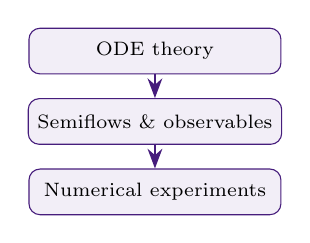
\begin{tikzpicture}[node distance=3mm, every node/.style={align=center,font=\scriptsize}]
\node[draw=LSUPurple,rounded corners,fill=SoftPurple,minimum width=3.2cm,minimum height=0.58cm] (theory) {ODE theory};
\node[draw=LSUPurple,rounded corners,fill=SoftPurple,below=of theory,minimum width=3.2cm,minimum height=0.58cm] (ops) {Semiflows \& observables};
\node[draw=LSUPurple,rounded corners,fill=SoftPurple,below=of ops,minimum width=3.2cm,minimum height=0.58cm] (num) {Numerical experiments};
\draw[-{Stealth[length=2.5mm]},thick,LSUPurple] (theory) -- (ops);
\draw[-{Stealth[length=2.5mm]},thick,LSUPurple] (ops) -- (num);
\end{tikzpicture}
\end{columns}
\end{frame}

% ------------------------------------------------------------
% 3. Roadmap
% ------------------------------------------------------------
\begin{frame}{Roadmap}
\begin{enumerate}
  \item \textbf{Well-posed autonomous systems and invariant regions}
  \begin{itemize}
    \item Picard--Lindel\"of and the local semiflow
    \item Nagumo's theorem and boundary tests for positive invariance
  \end{itemize}
  \item \textbf{Koopman--Lie viewpoint and operator splitting}
  \begin{itemize}
    \item local observable evolution and the generator \(Kg=\nabla g\cdot F\)
    \item natural coordinate splitting and the Lotka--Volterra laboratory
  \end{itemize}
  \item \textbf{Stopping times and finite-time blow-up}
  \begin{itemize}
    \item lower semicontinuity, domain exit, and blow-up
    \item Riccati lifting, first-zero detection, and computable Koopman eigenfunctions
  \end{itemize}
\end{enumerate}
\end{frame}

% ------------------------------------------------------------
% 4. Autonomous IVP and local semiflow
% ------------------------------------------------------------
\begin{frame}{Autonomous IVPs and Local Semiflows}
\small
Let
\[
\boxed{D\subset\R^n\text{ be open}},\qquad \boxed{F:D\to\R^n}
\]
and consider
\[
x'(t)=F(x(t)),\qquad x(0)=x\in D.
\]

For a unique maximal solution, write
\[
\flow(\cdot,x):[0,\mstop(x))\to D,
\qquad \mstop(x)\in(0,\infty].
\]

\begin{columns}[T,onlytextwidth]
\column{0.48\textwidth}
\begin{block}{Natural domain}
\[
\mathcal D
=
\{(t,x)\in[0,\infty)\times D:
0\le t<\mstop(x)\}.
\]
The solution map is \((t,x)\mapsto\flow(t,x)\).
\end{block}

\column{0.48\textwidth}
\begin{alertblock}{Semiflow structure}
\[
\flow(0,x)=x,
\qquad
\flow(t+s,x)=\flow(t,\flow(s,x))
\]
whenever both sides are defined.
\end{alertblock}
\end{columns}
\end{frame}

% ------------------------------------------------------------
% 5. Foundational theorems
% ------------------------------------------------------------
\begin{frame}{Picard--Lindel\"of: From an IVP to a Local Semiflow}
\small
Assume
\[
D\subset\R^n\text{ open},
\qquad
F:D\to\R^n\text{ locally Lipschitz}.
\]
Then every \(x\in D\) has a unique maximal solution
\[
\flow(\cdot,x):[0,\mstop(x))\to D.
\]

\begin{columns}[T,onlytextwidth]
\column{0.48\textwidth}
\begin{block}{Picard--Lindel\"of gives}
\footnotesize
\textbf{Existence}\par
A solution exists for each initial state.\par\vspace{0.4em}
\textbf{Uniqueness}\par
One initial state determines one trajectory.\par\vspace{0.4em}
\textbf{Continuous dependence}\par
Nearby initial states produce nearby trajectories on common admissible finite time intervals.
\end{block}

\column{0.48\textwidth}
\begin{alertblock}{Remaining lifetime}
For \(0\le t<\mstop(x)\),
\[
\boxed{\mstop(\flow(t,x))=\mstop(x)-t.}
\]
After flowing for time \(t\), exactly \(m(x)-t\) units of forward lifetime remain.
\end{alertblock}
\end{columns}
\end{frame}

\begin{frame}{Nagumo's Theorem in Koopman--Lie Form}
\footnotesize
Let \(\Omega\subset\R^n\) be closed with regular boundary,
\[
\Omega=\{x:g_j(x)\le0,\ j=1,\dots,r\},
\]
and let \(F\) be locally Lipschitz. With
\[
Kg_j(x)=\nabla g_j(x)\cdot F(x),
\]
the following are equivalent:
\begin{enumerate}
  \item \(\flow(t,x)\in\Omega\) for every \(x\in\Omega\) and every \(0\le t<\mstop(x)\);
  \item \(F(x)\in T_\Omega(x)\) for every \(x\in\partial\Omega\);
  \item \(Kg_j(x)\le0\) whenever \(g_j(x)=0\).
\end{enumerate}

\begin{alertblock}{Role in the defense}
Picard--Lindel\"of gives a well-defined trajectory; Nagumo gives the boundary test used to prove positive invariance.
\end{alertblock}
\end{frame}

% ------------------------------------------------------------
% 6. Finite maximal time
% ------------------------------------------------------------
\begin{frame}{What Finite Maximal Time Means}
\small
Under the Picard--Lindel\"of hypotheses, if \(\mstop(x)<\infty\), then for every compact set \(C\subset D\) there exists \(t_C<\mstop(x)\) such that
\[
\boxed{\flow(t,x)\notin C
\qquad\text{whenever }t_C<t<\mstop(x).}
\]

\vspace{0.5em}
\begin{columns}[T,onlytextwidth]
\column{0.48\textwidth}
\begin{tcolorbox}[colback=SoftPurple,colframe=LSUPurple,
  colbacktitle=LSUPurple,coltitle=white,title={Domain exit (bounded)},
  fonttitle=\bfseries,boxrule=0.9pt,arc=2mm,
  left=2mm,right=2mm,top=1.8mm,bottom=1.8mm]
\footnotesize
The trajectory stays bounded but approaches the boundary of its open state space.
\[
x'=1,\quad D=(-\infty,1),\quad x(0)=0.
\]
\[
\boxed{x(t)=t,\quad \mstop(0)=1.}
\]
\end{tcolorbox}

\column{0.48\textwidth}
\begin{tcolorbox}[colback=SoftPurple,colframe=LSUPurple,
  colbacktitle=LSUPurple,coltitle=white,title={Finite-time blow-up},
  fonttitle=\bfseries,boxrule=0.9pt,arc=2mm,
  left=2mm,right=2mm,top=1.8mm,bottom=1.8mm]
\footnotesize
On \(D=\R\), finite maximal time forces the solution to become unbounded.
\[
x'=x^2,\quad D=\R,\quad x(0)=1.
\]
\[
\boxed{x(t)=\frac{1}{1-t},\quad \mstop(1)=1.}
\]
\end{tcolorbox}
\end{columns}
\end{frame}

% ------------------------------------------------------------
% 7. Koopman-Lie
% ------------------------------------------------------------
\begin{frame}{Local Observable Evolution}
\small
Let \(g:D\to\R\) be an observable. For a \textbf{fixed} state \(x\in D\) and an admissible time
\[
0\le t<\mstop(x),
\]
define the pointwise Koopman action by
\[
\boxed{(T(t)g)(x)=g(\flow(t,x)).}
\]

For fixed \(x\) and \(t\), the dependence on the observable is linear:
\[
T(t)(a g_1+b g_2)(x)
=
a\,T(t)g_1(x)+b\,T(t)g_2(x).
\]

\begin{center}
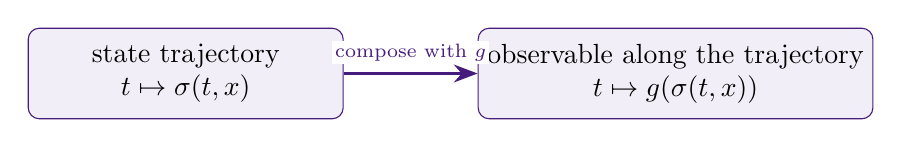
\begin{tikzpicture}[node distance=17mm]
\node[align=center,draw=LSUPurple,rounded corners,fill=SoftPurple,
      minimum width=4.0cm,minimum height=1.15cm] (state)
      {state trajectory\\\(t\mapsto \flow(t,x)\)};
\node[align=center,draw=LSUPurple,rounded corners,fill=SoftPurple,
      right=of state,minimum width=4.3cm,minimum height=1.15cm] (obs)
      {observable along the trajectory\\\(t\mapsto g(\flow(t,x))\)};
\draw[-{Stealth[length=3mm]},very thick,LSUPurple]
      (state.east) -- node[above=3pt,fill=white,inner sep=1pt,font=\scriptsize]{compose with \(g\)} (obs.west);
\end{tikzpicture}
\end{center}

\begin{alertblock}{Local-domain caveat}
The admissible time depends on \(x\). In this presentation we use the pointwise/local Koopman viewpoint and do not fix one particular Banach function space of observables.
\end{alertblock}
\end{frame}

% ------------------------------------------------------------
% 8. General coordinate-wise splitting
% ------------------------------------------------------------
\begin{frame}{The Koopman--Lie Generator Gives the Splitting Formula}
\footnotesize
For fixed \(x\), define the generator pointwise whenever the limit exists:
\[
Kg(x)
=
\lim_{t\downarrow0}
\frac{g(\flow(t,x))-g(x)}{t}.
\]
If \(g\) is differentiable,
\[
\boxed{Kg(x)=\nabla g(x)\cdot F(x).}
\]

For
\[
x'=F_1(x,y),\qquad y'=F_2(x,y),
\]
\[
\begin{aligned}
Kg(x,y)
&=g_xF_1+g_yF_2\\
&=:K_1g+K_2g.
\end{aligned}
\]
Thus
\[
\boxed{K=K_1+K_2.}
\]

\begin{alertblock}{Natural coordinate split}
\(K_1\) differentiates in \(x\) while \(y\) is a parameter; \(K_2\) differentiates in \(y\) while \(x\) is a parameter. In \(\R^n\), the same idea gives \(n\) pieces.
\end{alertblock}
\end{frame}

\begin{frame}{Coordinate Subflows}
\small
The generator split produces one-dimensional subproblems.

\begin{columns}[T,onlytextwidth]
\column{0.48\textwidth}
\begin{block}{\(K_1\): evolve \(x\)}
Freeze \(y\) as a parameter:
\[
x'=F_1(x,y),\qquad x(0)=v.
\]
If its solution is \(\sigma_1(t,v;y)\), then
\[
\boxed{\Phi_1^t(x,y)=\bigl(\sigma_1(t,x;y),y\bigr).}
\]
\end{block}

\column{0.48\textwidth}
\begin{block}{\(K_2\): evolve \(y\)}
Freeze \(x\) as a parameter:
\[
y'=F_2(x,y),\qquad y(0)=w.
\]
If its solution is \(\sigma_2(t,w;x)\), then
\[
\boxed{\Phi_2^t(x,y)=\bigl(x,\sigma_2(t,y;x)\bigr).}
\]
\end{block}
\end{columns}

\begin{center}
\small Partial differentiation explains the ``freezing'': the other coordinates are carried along as parameters.
\end{center}
\end{frame}

% ------------------------------------------------------------
% 9. Koopman order reversal
% ------------------------------------------------------------
\begin{frame}{State Composition vs. Koopman Composition}
\small
One Lie--Trotter state step is
\[
\boxed{z_{k+1}=\Phi_2^h(\Phi_1^h(z_k))},
\]
so the state composition is \(\Phi_2^h\circ\Phi_1^h\).

For admissible \(h\),
\[
(T_i(h)f)(z)=f(\Phi_i^h(z)).
\]
Hence
\[
\begin{aligned}
(T_1(h)T_2(h)f)(z)
&=T_1(h)(f\circ\Phi_2^h)(z)\\
&=f(\Phi_2^h(\Phi_1^h(z))),
\end{aligned}
\]
and therefore
\[
\boxed{T_{\Phi_2^h\circ\Phi_1^h}=T_1(h)T_2(h).}
\]

\end{frame}

% ------------------------------------------------------------
% 10. LV system and positivity
% ------------------------------------------------------------
\begin{frame}{Lotka--Volterra: Nagumo Check for the Nonnegative Quadrant}
\scriptsize
Consider
\[
x'=\alpha x-\beta xy,\qquad
y'=\delta xy-\tau y.
\]
The closed biologically meaningful region is
\[
\Omega_+=\{(x,y):x\ge0,\ y\ge0\}.
\]
Set
\[
g_1(x,y)=-x,\qquad g_2(x,y)=-y,
\]
so
\[
\nabla g_1=(-1,0),\qquad \nabla g_2=(0,-1).
\]
Hence, using \(Kg_j=\nabla g_j\cdot F\),
\[
Kg_1=\beta xy-\alpha x,\qquad
Kg_2=\tau y-\delta xy.
\]
On the active boundaries,
\[
x=0\Rightarrow Kg_1=0,
\qquad
y=0\Rightarrow Kg_2=0.
\]
Therefore
\[
\boxed{\Omega_+\text{ is positively invariant}.}
\]

\begin{alertblock}{Important distinction}
Nagumo gives invariance of the closed nonnegative quadrant; strict positivity needs a separate argument.
\end{alertblock}
\end{frame}

% ------------------------------------------------------------
% 11. LV Hamiltonian
% ------------------------------------------------------------
\begin{frame}{Strict Positivity and the Conserved Quantity \(H\)}
\footnotesize
For positive initial data,
\[
x'=x(\alpha-\beta y),\qquad
y'=y(\delta x-\tau),
\]
so
\[
x(t)=x_0\exp\!\left(\int_0^t(\alpha-\beta y(s))\,ds\right)>0,
\]
\[
y(t)=y_0\exp\!\left(\int_0^t(\delta x(s)-\tau)\,ds\right)>0.
\]

Therefore the logarithms in
\[
\boxed{H(x,y)=\delta x-\tau\ln x+\beta y-\alpha\ln y}
\]
remain defined. Direct differentiation gives
\[
\boxed{\frac{d}{dt}H(x(t),y(t))=0.}
\]

\begin{center}
\textbf{\textcolor{LSUPurple}{Numerical diagnostic:}} compare methods by their relative error in the conserved quantity \(H\).
\end{center}
\end{frame}

% ------------------------------------------------------------
% 12. LV splitting updates
% ------------------------------------------------------------
\begin{frame}{Lie--Trotter and Strang Updates for Lotka--Volterra}
Freezing \(y\) gives
\[
  \sigma(t,x;y)=xe^{t(\alpha-\beta y)},
\]
and freezing \(x\) gives
\[
  \gamma(t,y;x)=ye^{t(\delta x-\tau)}.
\]

\begin{columns}[T,onlytextwidth]
\column{0.48\textwidth}
\begin{block}{One Lie--Trotter step}
\[
 x_{k+1}=x_k e^{h(\alpha-\beta y_k)},
\]
\[
 y_{k+1}=y_k e^{h(\delta x_{k+1}-\tau)}.
\]
\end{block}
\column{0.48\textwidth}
\begin{block}{One Strang step}
\[
 x_{k+1/2}=x_k e^{\frac h2(\alpha-\beta y_k)},
\]
\[
 y_{k+1}=y_k e^{h(\delta x_{k+1/2}-\tau)},
\]
\[
 x_{k+1}=x_{k+1/2}e^{\frac h2(\alpha-\beta y_{k+1})}.
\]
\end{block}
\end{columns}
\end{frame}

% ------------------------------------------------------------
% 13. Numerical setup
% ------------------------------------------------------------
\begin{frame}{Baseline Numerical Experiment}
\small
\begin{columns}[T,onlytextwidth]
\column{0.48\textwidth}
\begin{block}{Parameters}
\[
\alpha=1.5,\quad \beta=1,\quad \delta=1,\quad \tau=3,
\]
\[
x(0)=10,\qquad y(0)=5,
\]
\[
0\le t\le30,\qquad h=0.01.
\]
\end{block}
The exact conserved value is
\[
H_0:=H(x_0,y_0)\approx5.6780878524.
\]

\column{0.48\textwidth}
\begin{alertblock}{Methods compared}
\begin{itemize}
  \item \textbf{Forward Euler},
  \item Lie--Trotter splitting,
  \item Strang splitting,
  \item adaptive \texttt{solve\_ivp} reference solution.
\end{itemize}
\end{alertblock}

Final signed relative error in \(H\):
\[
\boxed{
100\,\frac{H(x_n,y_n)-H_0}{H_0}.
}
\]
\end{columns}
\end{frame}

% ------------------------------------------------------------
% 14. LV visual result
% ------------------------------------------------------------
\begin{frame}{Baseline Simulation: Relative Error in \(H\)}
\centering
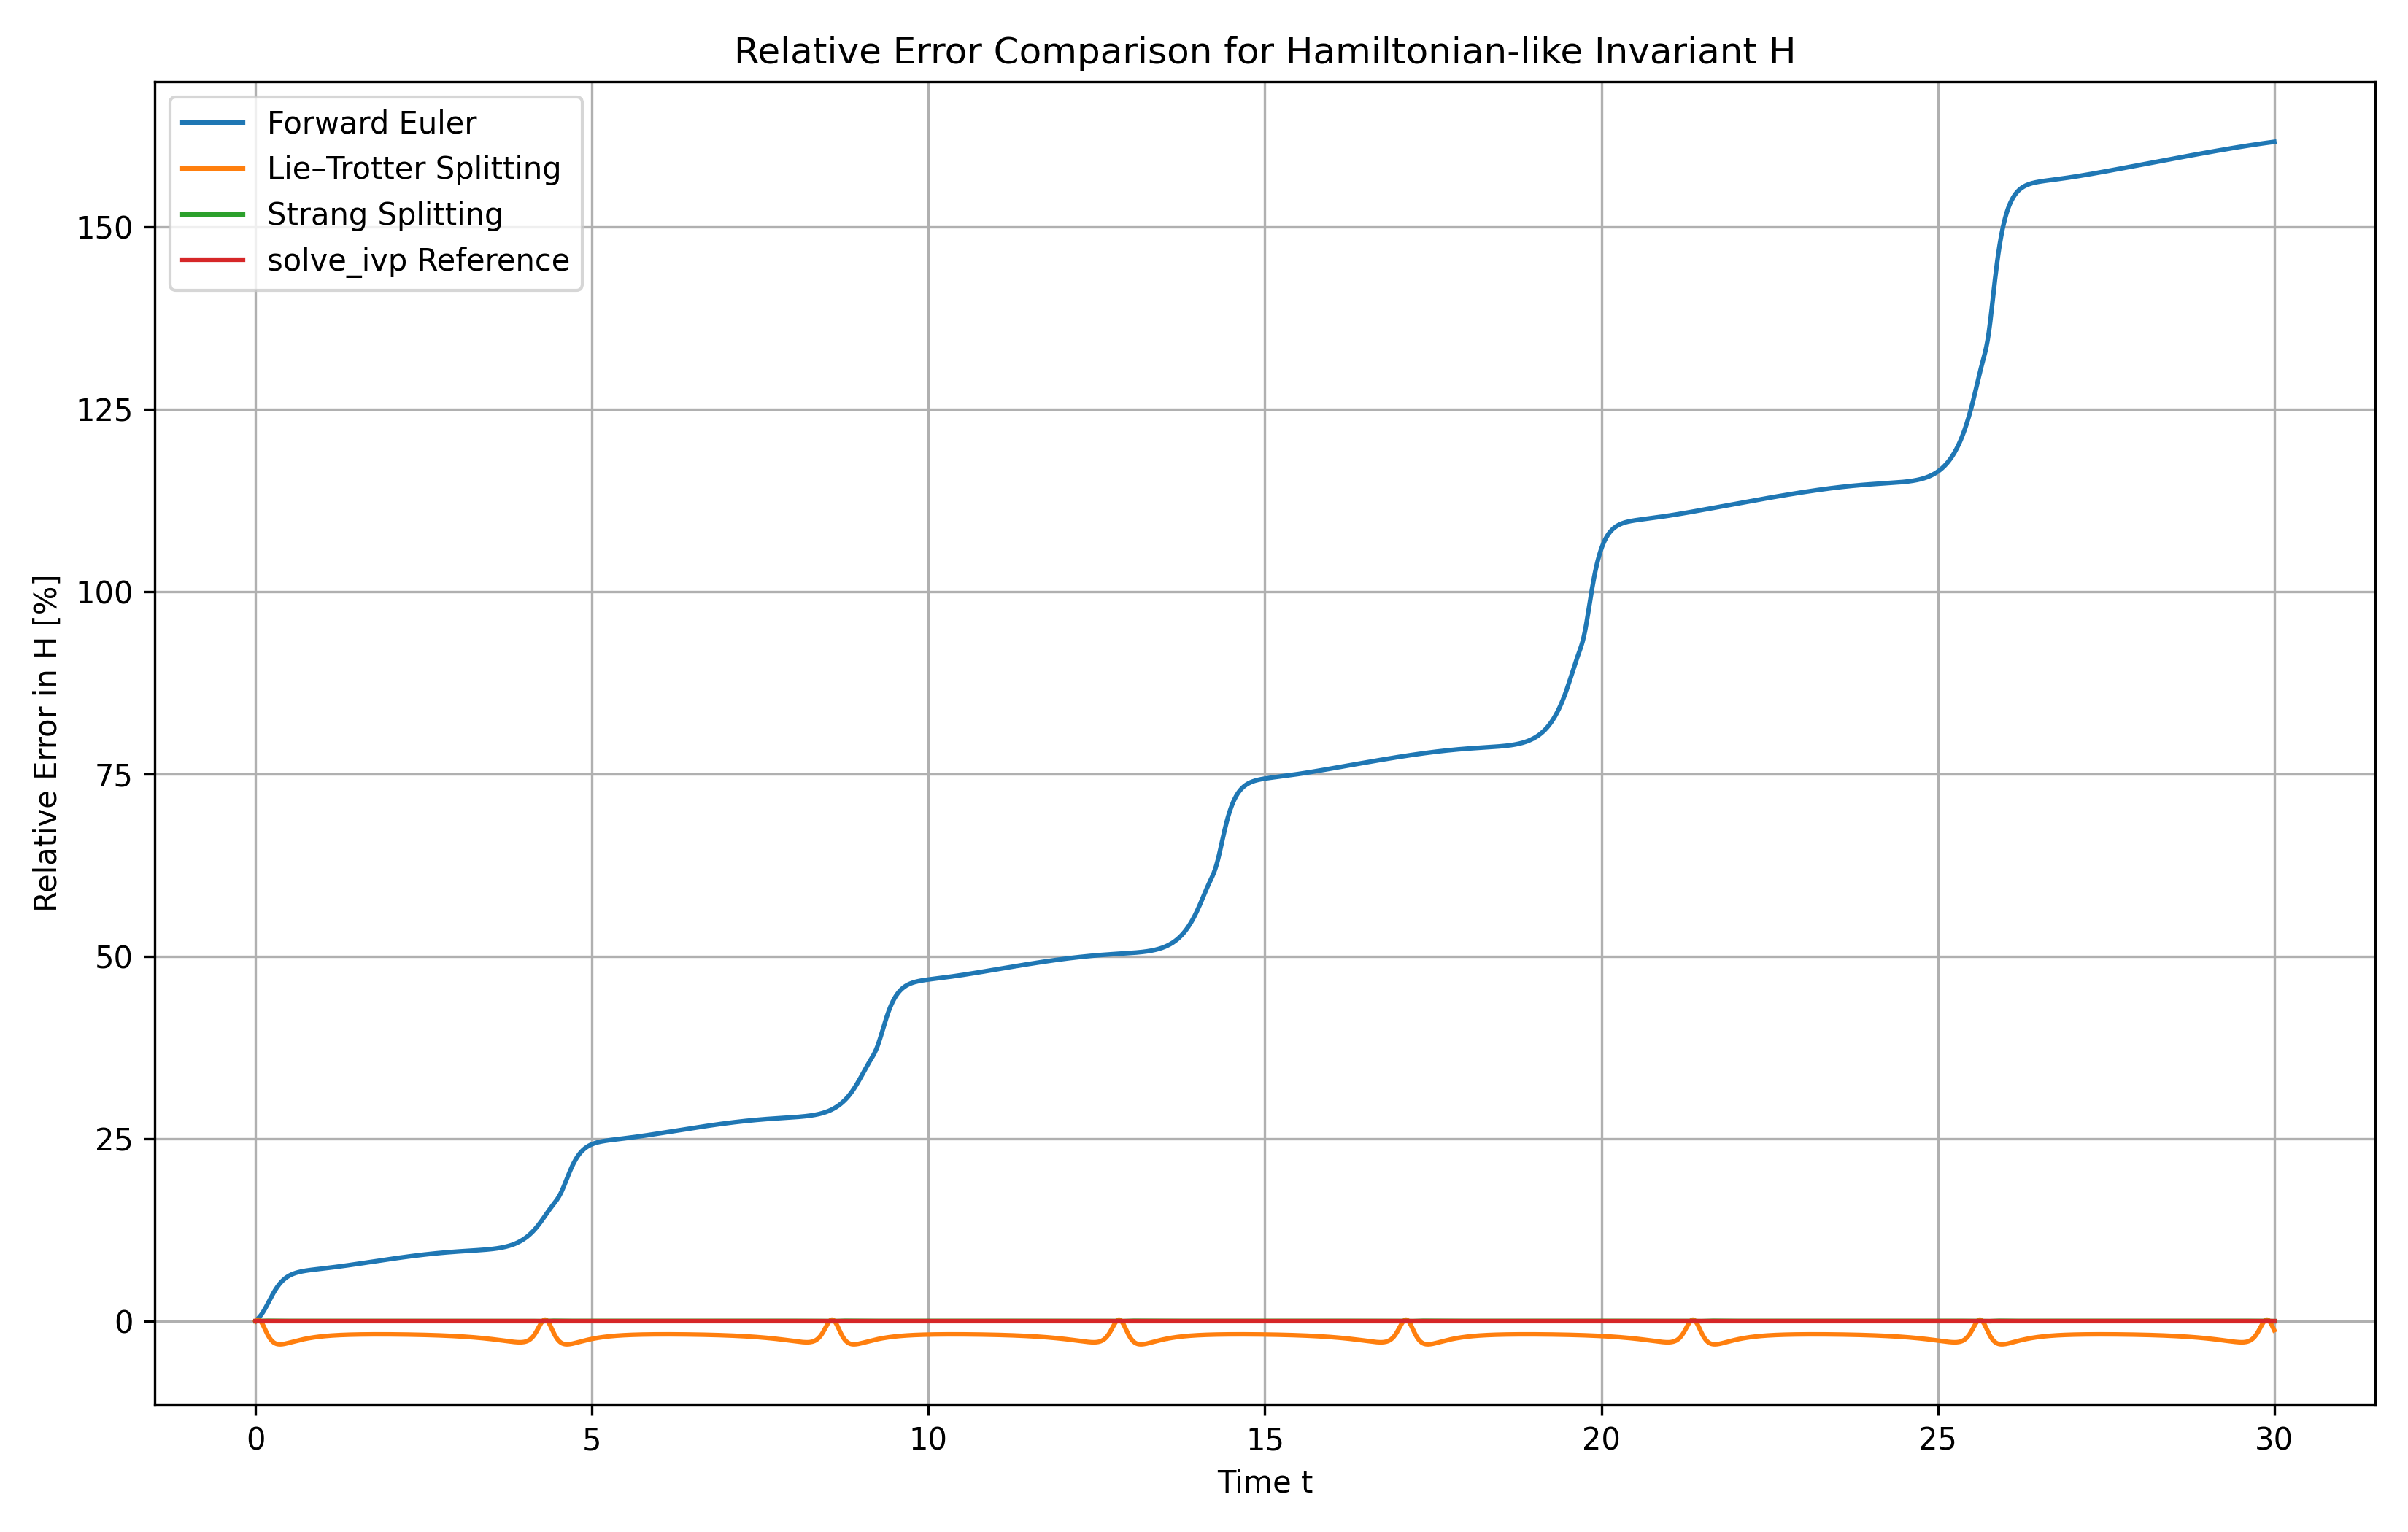
\includegraphics[height=0.63\textheight,keepaspectratio]{beamer_assets/lv_relative_error.png}

\vspace{0.1em}
\scriptsize
\textbf{\textcolor{LSUPurple}{Interpretation:}}
the exact flow preserves \(H\), so departures from zero measure numerical error in this conserved quantity.
\end{frame}

\begin{frame}{Baseline Simulation: Phase Portrait}
\centering
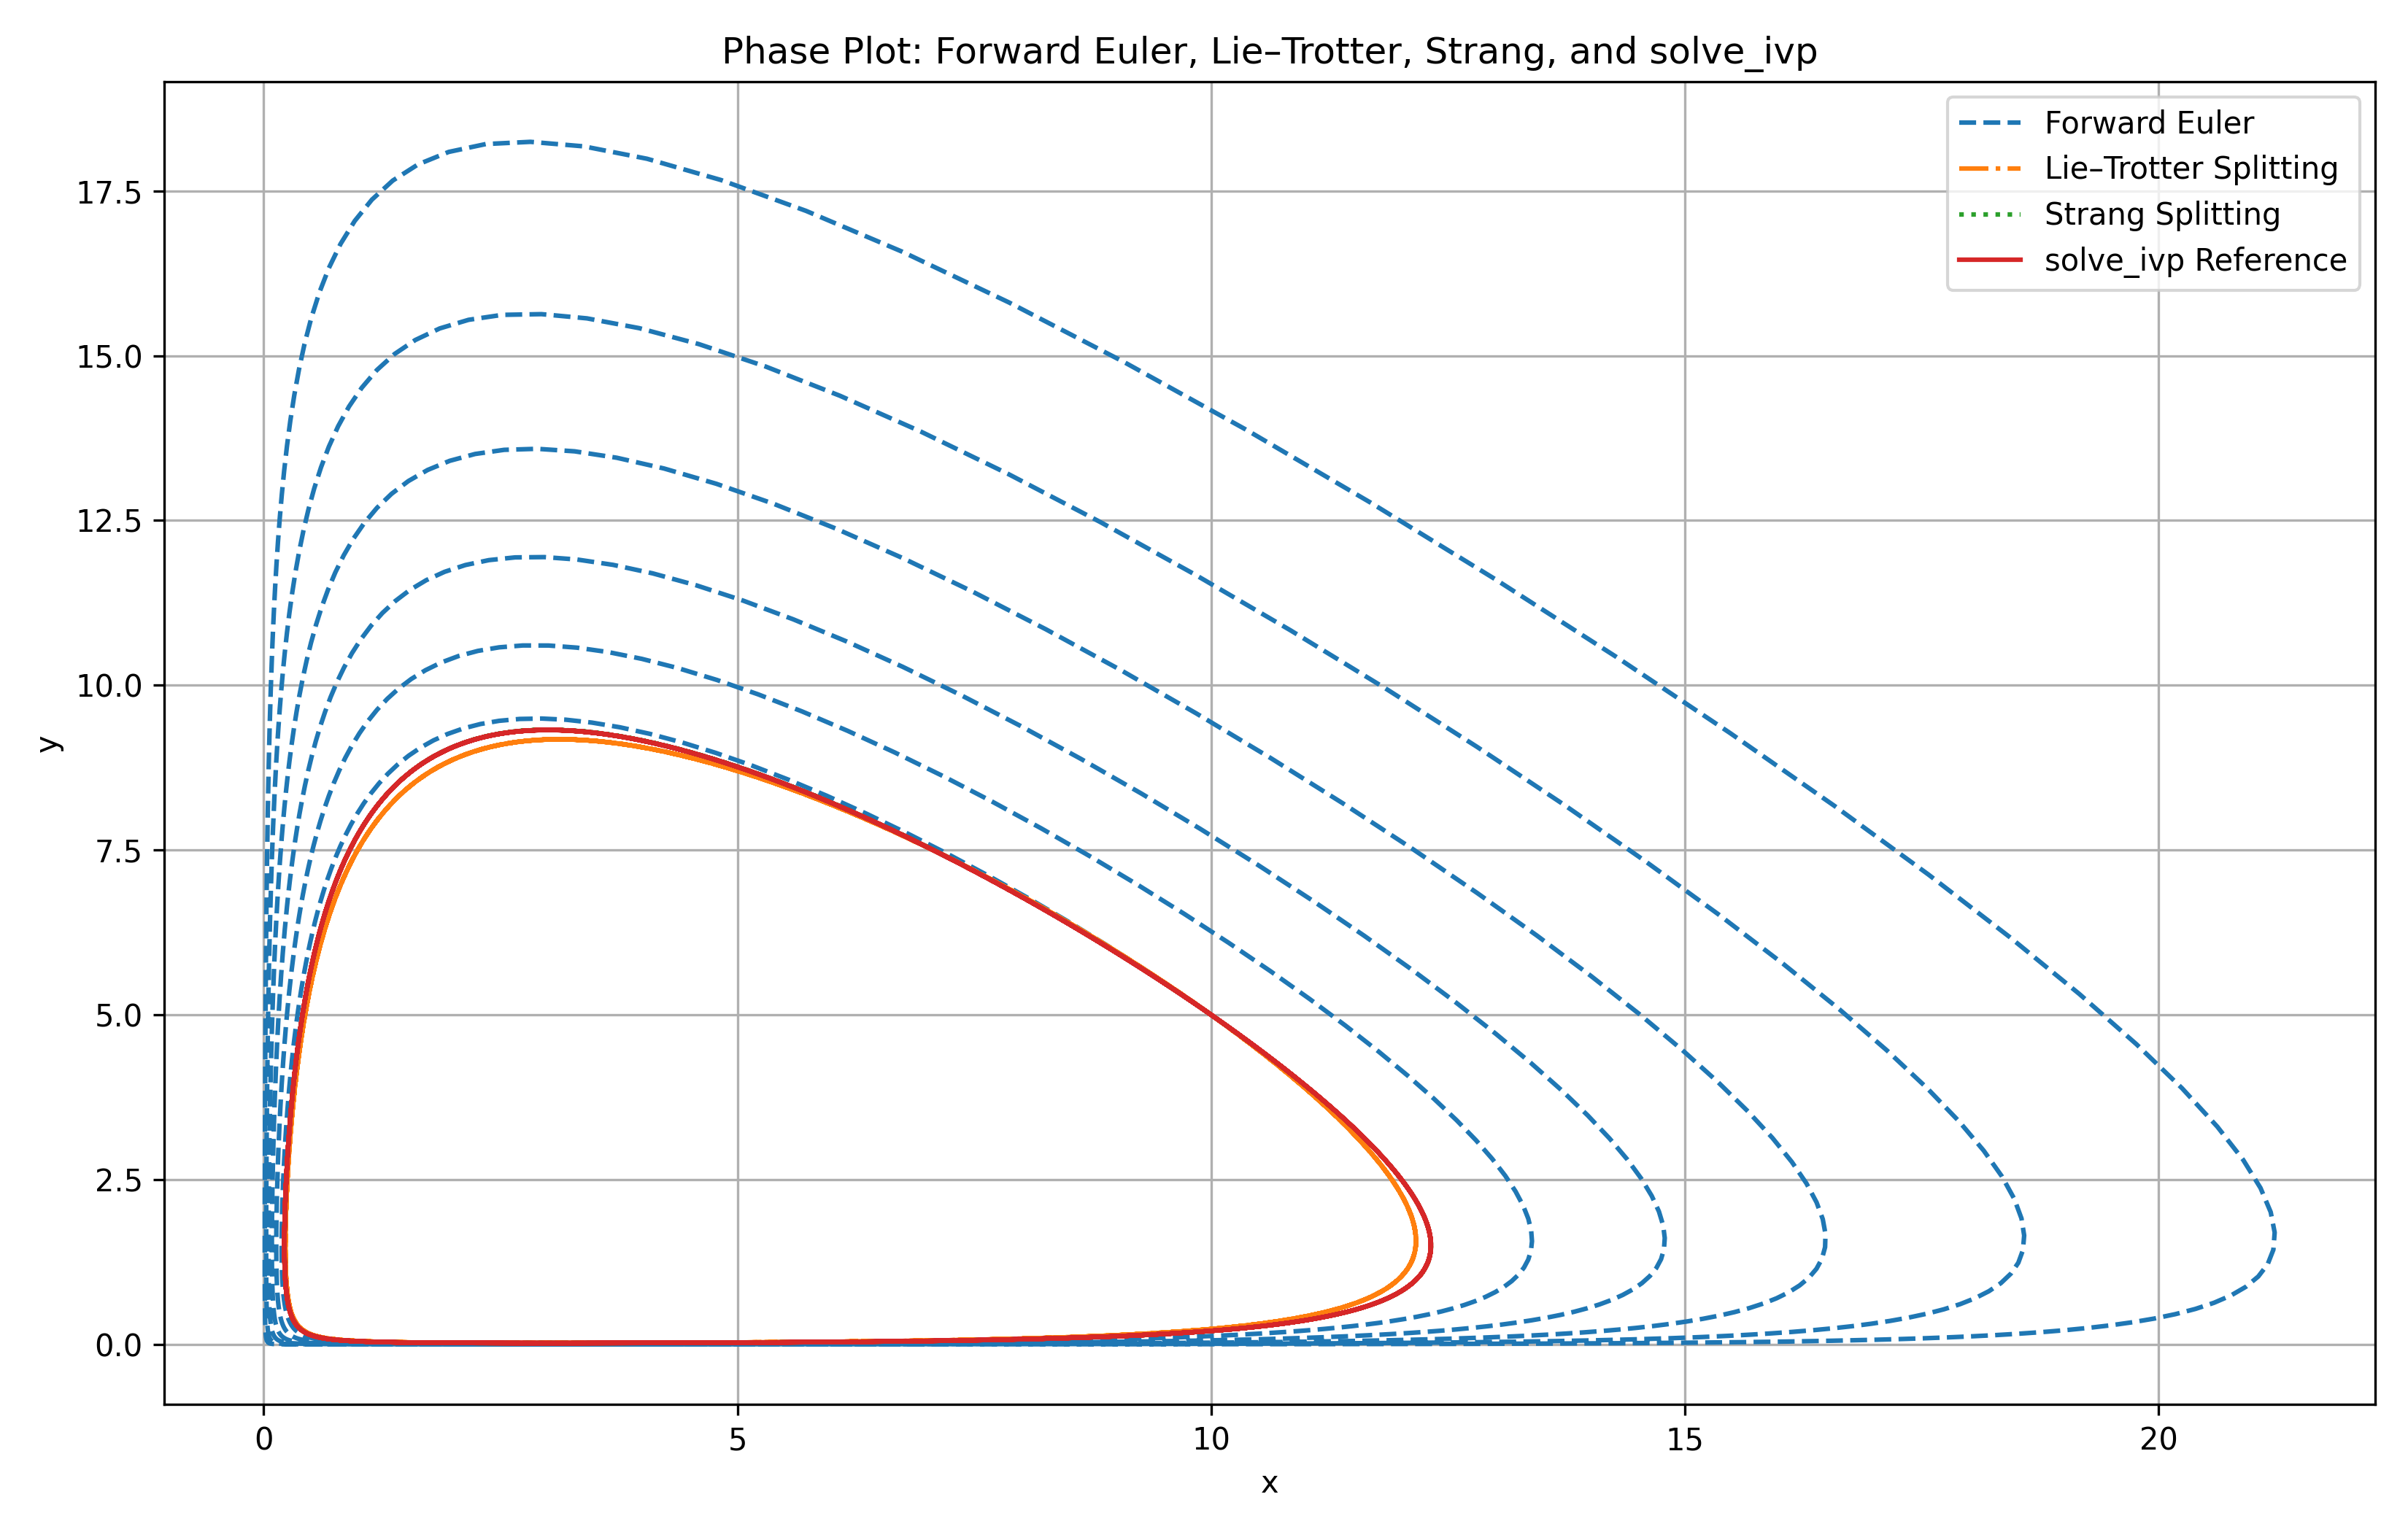
\includegraphics[height=0.63\textheight,keepaspectratio]{beamer_assets/lv_phase_plot.png}

\vspace{0.1em}
\scriptsize
\textbf{\textcolor{LSUPurple}{Why both views matter:}}
trajectories can look qualitatively similar while the relative error in \(H\) differs substantially.
\end{frame}

% ------------------------------------------------------------
% 15. Baseline table
% ------------------------------------------------------------
\begin{frame}{Baseline Final Relative Error in \(H\)}
\centering
\begin{tabular}{lr}
\toprule
\textbf{Method} & \textbf{Final signed relative error in \(H\)} \\
\midrule
Forward Euler & \(161.6626980950\%\) \\
Lie--Trotter & \(-1.2478784951\%\) \\
Strang & \(-0.0023496487\%\) \\
\texttt{solve\_ivp} & \(-0.0000001293\%\) \\
\bottomrule
\end{tabular}

\vspace{0.7em}
\begin{block}{Interpretation}
This table compares the particular implementations used in the numerical laboratory. It shows how well each run preserves \(H\); it is \emph{not} a ranking of all possible splitting methods.
\end{block}
\end{frame}

% ------------------------------------------------------------
% Restored to main talk: step-size refinement (backup copy retained)
% ------------------------------------------------------------
\begin{frame}{Step-Size Refinement: Relative Error in \(H\)}
\centering
\scriptsize
\setlength{\tabcolsep}{3.0pt}
\renewcommand{\arraystretch}{1.4}
\begin{tabular}{ccccc}
\toprule
\(h\) & Forward Euler & Lie--Trotter & Strang & \texttt{solve\_ivp} \\
\midrule
0.01  & 161.6626980950\% & -1.2478784951\% & -0.0023496487\% & -0.0000001293\% \\
0.005 & 67.7244617696\%  &  0.1034928563\% & -0.0006536800\% & -0.0000001293\% \\
0.001 & 10.3619531982\%  & -0.0865717147\% & -0.0000269765\% & -0.0000001293\% \\
\bottomrule
\end{tabular}

\vspace{0.8em}
\begin{block}{What refinement shows}
\footnotesize
At the tested step sizes, reducing \(h\) reduces the \emph{magnitude} of the final relative error in \(H\) for all three fixed-step methods. Lie--Trotter's signed error changes sign, so compare magnitudes rather than signed values.
\end{block}
\begin{alertblock}{Adaptive reference}
\footnotesize
\texttt{solve\_ivp} chooses its own internal steps from error tolerances; the listed \(h\) controls the fixed-step methods, not its internal step size.
\end{alertblock}
\end{frame}

% ------------------------------------------------------------
% 16. Step-size effects
% ------------------------------------------------------------
\begin{frame}{How to Interpret the Numerical Comparison}
\small
\begin{itemize}
  \item \textbf{Forward Euler} is included as a simple first-order baseline.
  \item The Lie--Trotter and Strang schemes used here are \textbf{low-order splitting methods}.
  \item \texttt{solve\_ivp} is an \textbf{adaptive high-accuracy reference solver}; it chooses internal steps using error tolerances.
  \item The \(h\) in the fixed-step experiments directly controls forward Euler, Lie--Trotter, and Strang, but does not play the same role for \texttt{solve\_ivp}.
  \item \textbf{Higher-order splitting methods also exist} and can achieve much greater accuracy; the baseline table should not be read as evidence that splitting is inherently inferior.
\end{itemize}

\begin{alertblock}{Scope of this thesis}
The purpose of the experiment is to implement the methods and use conservation of \(H\) as a structural diagnostic, not to establish a comprehensive numerical ranking.
\end{alertblock}
\end{frame}

% ------------------------------------------------------------
% 17. Transition to stopping times
% ------------------------------------------------------------
\begin{frame}{Stopping Times and Lower Semicontinuity}
\small
The stopping-time function is
\[
\boxed{\mstop:D\to(0,\infty].}
\]
For a maximal solution,
\[
\flow(\cdot,x):[0,\mstop(x))\to D.
\]

It is \textbf{lower semicontinuous}: if \(x_n\to x\), then
\[
\boxed{\mstop(x)\le \liminf_{n\to\infty}\mstop(x_n).}
\]

\begin{columns}[T,onlytextwidth]
\column{0.47\textwidth}
\begin{block}{What this permits}
Nearby states may have \emph{larger} lifetimes, even \(+\infty\).
\end{block}
\column{0.47\textwidth}
\begin{alertblock}{What it prevents}
Nearby states cannot suddenly have substantially \emph{smaller} maximal lifetimes.
\end{alertblock}
\end{columns}

\vspace{0.2em}
Finite stopping time can arise either by \textbf{domain exit} or by genuine \textbf{finite-time blow-up}.
\end{frame}

% ------------------------------------------------------------
% 18. Discontinuous stopping-time example
% ------------------------------------------------------------
\begin{frame}{Example 3: A Discontinuous Stopping-Time Function}
\footnotesize
Remove the ray
\[
\Gamma=\{(x,0):x\ge1\},
\qquad
\Omega=\R^2\setminus\Gamma,
\]
and use
\[
F(x,y)=(1,0),\qquad z(t;z_0)=(x_0+t,y_0).
\]
The stopping time is an extended-real-valued function
\[
\mstop:\Omega\to(0,\infty],
\]
with
\[
\mstop(x_0,y_0)=
\begin{cases}
+\infty, & y_0\neq0,\\
1-x_0, & y_0=0,\ x_0<1.
\end{cases}
\]
Fix \(x_0<1\). If
\[
z_n=\left(x_0,\frac1n\right)\to(x_0,0),
\]
then \(m(z_n)=+\infty\) while \(m(x_0,0)=1-x_0<\infty\).

\begin{center}
\textbf{\textcolor{LSUPurple}{Conclusion:}}
\(m\) is not continuous, but the jump is upward, so lower semicontinuity is preserved.
\end{center}
\end{frame}

% ------------------------------------------------------------
% 19. Blow-up example
% ------------------------------------------------------------
\begin{frame}{Example 4: Nagumo Check for the Negative Quadrant}
\small
Consider
\[
x'=y-x^2,\qquad y'=x-y,
\]
and
\[
Q_-=\{(x,y):x\le0,\ y\le0\}.
\]
Set
\[
g_1(x,y)=x,\qquad g_2(x,y)=y,
\]
so
\[
\nabla g_1=(1,0),\qquad \nabla g_2=(0,1).
\]
Hence, using \(Kg_j=\nabla g_j\cdot F\),
\[
Kg_1=y-x^2,\qquad Kg_2=x-y.
\]
On the active boundaries,
\[
x=0\Rightarrow Kg_1=y\le0,
\qquad
y=0\Rightarrow Kg_2=x\le0.
\]
Therefore Nagumo gives
\[
\boxed{Q_-\text{ is positively invariant}.}
\]
\end{frame}

\begin{frame}{Example 4: Blow-up Estimate in the Invariant Region}
\begin{columns}[T,onlytextwidth]
\column{0.34\textwidth}
\scriptsize
Inside \(Q_-\),
\[
x'=y-x^2\le -x^2.
\]
Compare with
\[
z'=-z^2,\qquad z(0)=x_0<0,
\]
whose solution is
\[
z(t)=\frac{x_0}{1+x_0t}.
\]
It blows up at \(t=1/|x_0|\), so
\[
\boxed{\mstop(x_0,y_0)\le\frac1{|x_0|}}.
\]

\column{0.64\textwidth}
\centering
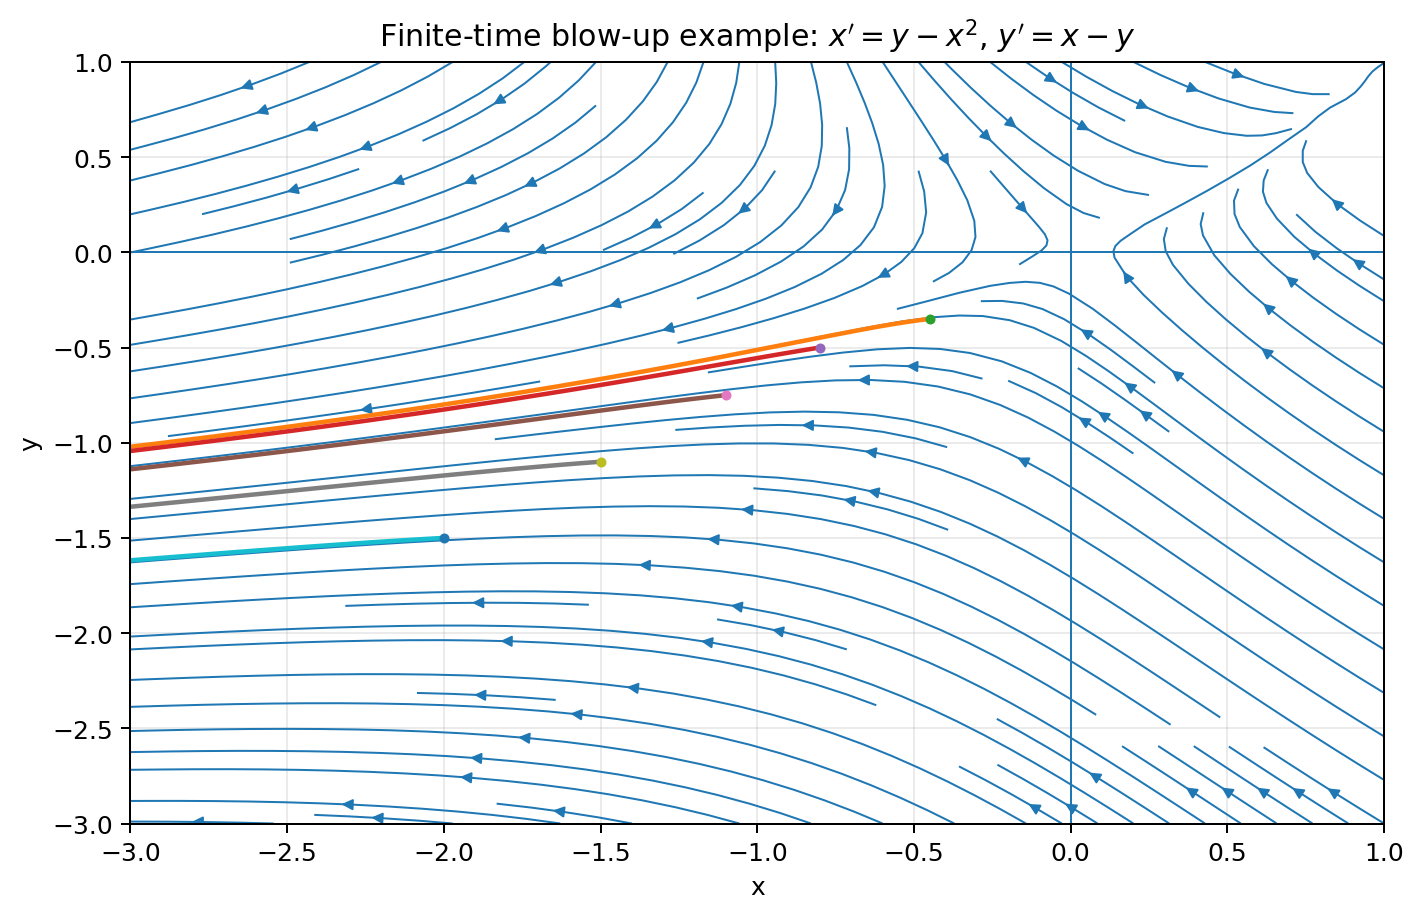
\includegraphics[width=\linewidth,height=0.58\textheight,keepaspectratio]{beamer_assets/koopman_blowup_phase.png}
\end{columns}
\end{frame}

% ------------------------------------------------------------
% 20. Koopman eigenfunction
% ------------------------------------------------------------
\begin{frame}{The Remaining Lifetime as an Observable}
\small
The remaining-lifetime identity is
\[
\mstop(\flow(t,x))=\mstop(x)-t,
\qquad 0\le t<\mstop(x).
\]
Define
\[
\boxed{\phi(x)=e^{-\mstop(x)}},
\qquad e^{-\infty}:=0.
\]
Then, pointwise for admissible \(t\),
\[
\begin{aligned}
\phi(\flow(t,x))
&=e^{-\mstop(\flow(t,x))}\\
&=e^{-(\mstop(x)-t)}
=e^t\phi(x).
\end{aligned}
\]

\[
\boxed{\phi(\flow(t,x))=e^t\phi(x).}
\]

\begin{alertblock}{Interpretation}
\(\phi\ge0\) everywhere and is strictly positive wherever the forward lifetime is finite. Formally, on the generator domain, \(K\phi=\phi\).
\end{alertblock}
\end{frame}

% ------------------------------------------------------------
% 21. Lifting Riccati
% ------------------------------------------------------------
\begin{frame}{Lifting a Non-autonomous Riccati Equation}
\small
Start with
\[
u'(t)=t^2+u(t)^2,
\qquad
u(s)=y.
\]
Introduce autonomous time \(\tau\):
\[
\boxed{
\begin{aligned}
x'(\tau)&=1,\\
w'(\tau)&=x(\tau)^2+w(\tau)^2,
\end{aligned}}
\qquad
(x(0),w(0))=(s,y).
\]
Then
\[
x(\tau)=s+\tau,
\qquad
w(\tau)=u(s+\tau).
\]

\begin{alertblock}{Why lift?}
The non-autonomous scalar equation becomes an autonomous system on \(\R^2\), so the local semiflow and stopping-time framework applies directly.
\end{alertblock}
\end{frame}

% ------------------------------------------------------------
% 22. Comparison and finiteness
% ------------------------------------------------------------
\begin{frame}{The Riccati Stopping Time Is Finite for Every Initial Condition}
\footnotesize
For \(y>0\),
\[
\boxed{\mstop(s,y)\le\frac1y}
\]
by comparison with \(z'=z^2\).

For arbitrary \((s,y)\),
\[
w'(\tau)\ge(s+\tau)^2,
\]
so
\[
w(\tau)
\ge
y+\frac{(s+\tau)^3-s^3}{3}.
\]
Choose \(\tau_1>0\) so the right-hand side is positive. Then \(w(\tau_1)>0\), and from that time onward
\[
w'(\tau)\ge w(\tau)^2.
\]
Comparison with \(z'=z^2\) now forces finite-time blow-up.

\[
\boxed{\mstop(s,y)<\infty
\qquad\text{for every }(s,y)\in\R^2.}
\]
\end{frame}

% ------------------------------------------------------------
% 23. Riccati linearization
% ------------------------------------------------------------
\begin{frame}{Riccati Linearization}
\small
Fix \((s,y)\in\R^2\). For \(x\ge s\),
\[
u'(x)=x^2+u(x)^2,\qquad u(s)=y.
\]

Use the Riccati substitution
\[
\boxed{u(x)=-\frac{v'(x)}{v(x)}}.
\]

This converts the nonlinear equation into the linear second-order IVP
\[
\boxed{
\begin{cases}
v''(x)+x^2v(x)=0,\\
v(s)=1,\\
v'(s)=-y,
\end{cases}
\qquad x\ge s.}
\]

\begin{alertblock}{Main point}
The Riccati substitution replaces the nonlinear blow-up problem with a linear second-order equation whose zeros can be studied directly.
\end{alertblock}
\end{frame}

% ------------------------------------------------------------
% 24. First zero and blow-up
% ------------------------------------------------------------
\begin{frame}{The First Zero Determines the Maximal Lifetime}
\small
Let \(\xi_*(s,y)>s\) be the first zero to the right of \(s\) of
\[
v''(x)+x^2v(x)=0,
\qquad
v(s)=1,\quad v'(s)=-y.
\]
Sturm comparison guarantees that such a zero exists.

As long as \(v(x)\neq0\),
\[
u(x)=-\frac{v'(x)}{v(x)}
\]
recovers the Riccati solution. The first zero is simple, so this quotient has a pole at \(x=\xi_*\); hence the Riccati solution blows up there.

Since \(x=s+\tau\),
\[
\boxed{\mstop(s,y)=\xi_*(s,y)-s.}
\]

\begin{alertblock}{Key distinction}
\(\xi_*\) is the physical blow-up location; \(m(s,y)\) is the elapsed forward lifetime.
\end{alertblock}
\end{frame}

% ------------------------------------------------------------
% 25. Event detection
% ------------------------------------------------------------
\begin{frame}{Numerical Computation by Event Detection}
\small
Rewrite the linear equation as
\[
v'=p,
\qquad
p'=-x^2v,
\qquad
v(s)=1,\quad p(s)=-y.
\]

\begin{columns}[T,onlytextwidth]
\column{0.48\textwidth}
\begin{block}{Numerical procedure}
Use \texttt{solve\_ivp} on the linear system and define the event
\[
E(x,v,p)=v.
\]
Stop when the first zero is detected.
\end{block}

\column{0.48\textwidth}
\begin{alertblock}{Convert zero to lifetime}
If the detected first zero is \(\widehat{\xi}_*\), then
\[
\boxed{\widehat m(s,y)=\widehat{\xi}_*-s.}
\]
The computation avoids introducing an arbitrarily large threshold for the nonlinear solution.
\end{alertblock}
\end{columns}

\vspace{0.25em}
\centering
The numerical event is an approximation of the theoretical first zero \(\xi_*\).
\end{frame}

% ------------------------------------------------------------
% 26. Numerical Riccati result
% ------------------------------------------------------------
\begin{frame}{Example 5: First Zero of the Linearized Solution}
\scriptsize
For \(s=0,\ y=1\), solve
\[
v''+x^2v=0,\qquad v(0)=1,\qquad v'(0)=-1.
\]
Event detection gives
\[
\boxed{\xi_*\approx0.969810653960,\qquad m(0,1)=\xi_*.}
\]

\centering
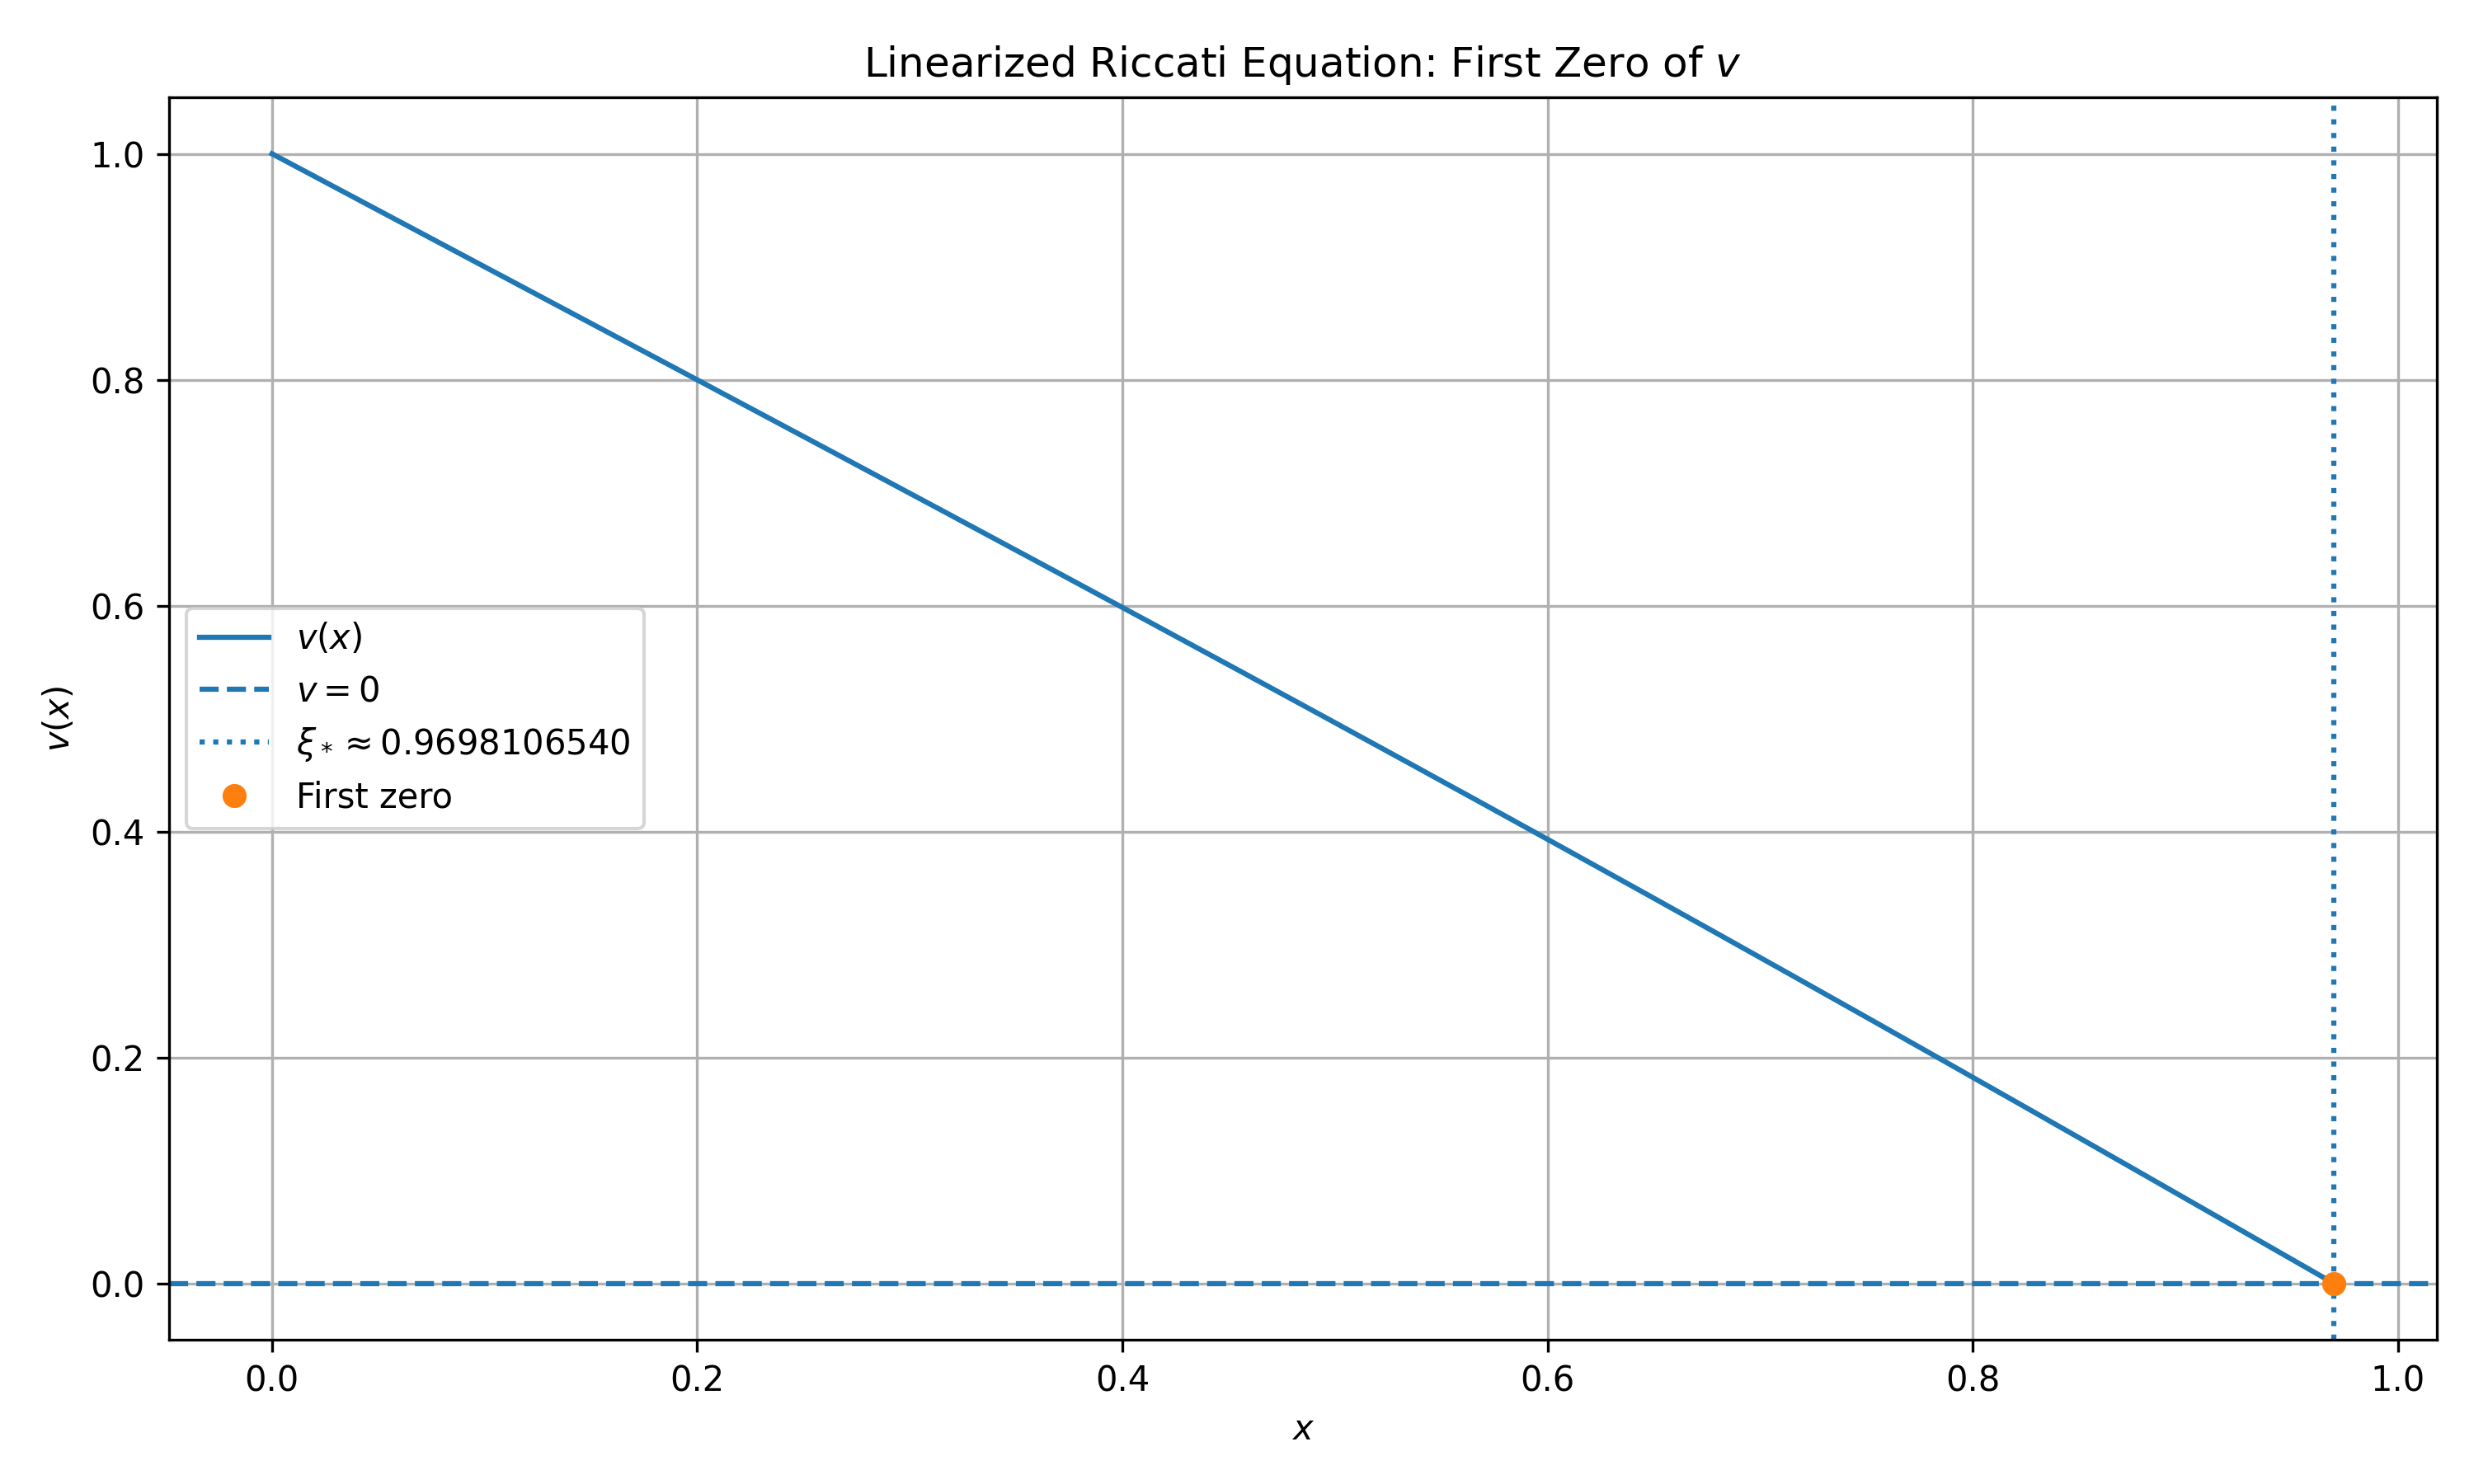
\includegraphics[height=0.50\textheight,keepaspectratio]{beamer_assets/riccati_linear_zero.png}
\end{frame}

\begin{frame}{Example 5: Reconstructed Riccati Blow-up}
\scriptsize
Reconstruct
\[
u(x)=-\frac{v'(x)}{v(x)}.
\]
As \(x\uparrow\xi_*\), \(u(x)\) grows rapidly:
\[
\boxed{m(0,1)\approx0.969810653960<1.}
\]

\centering
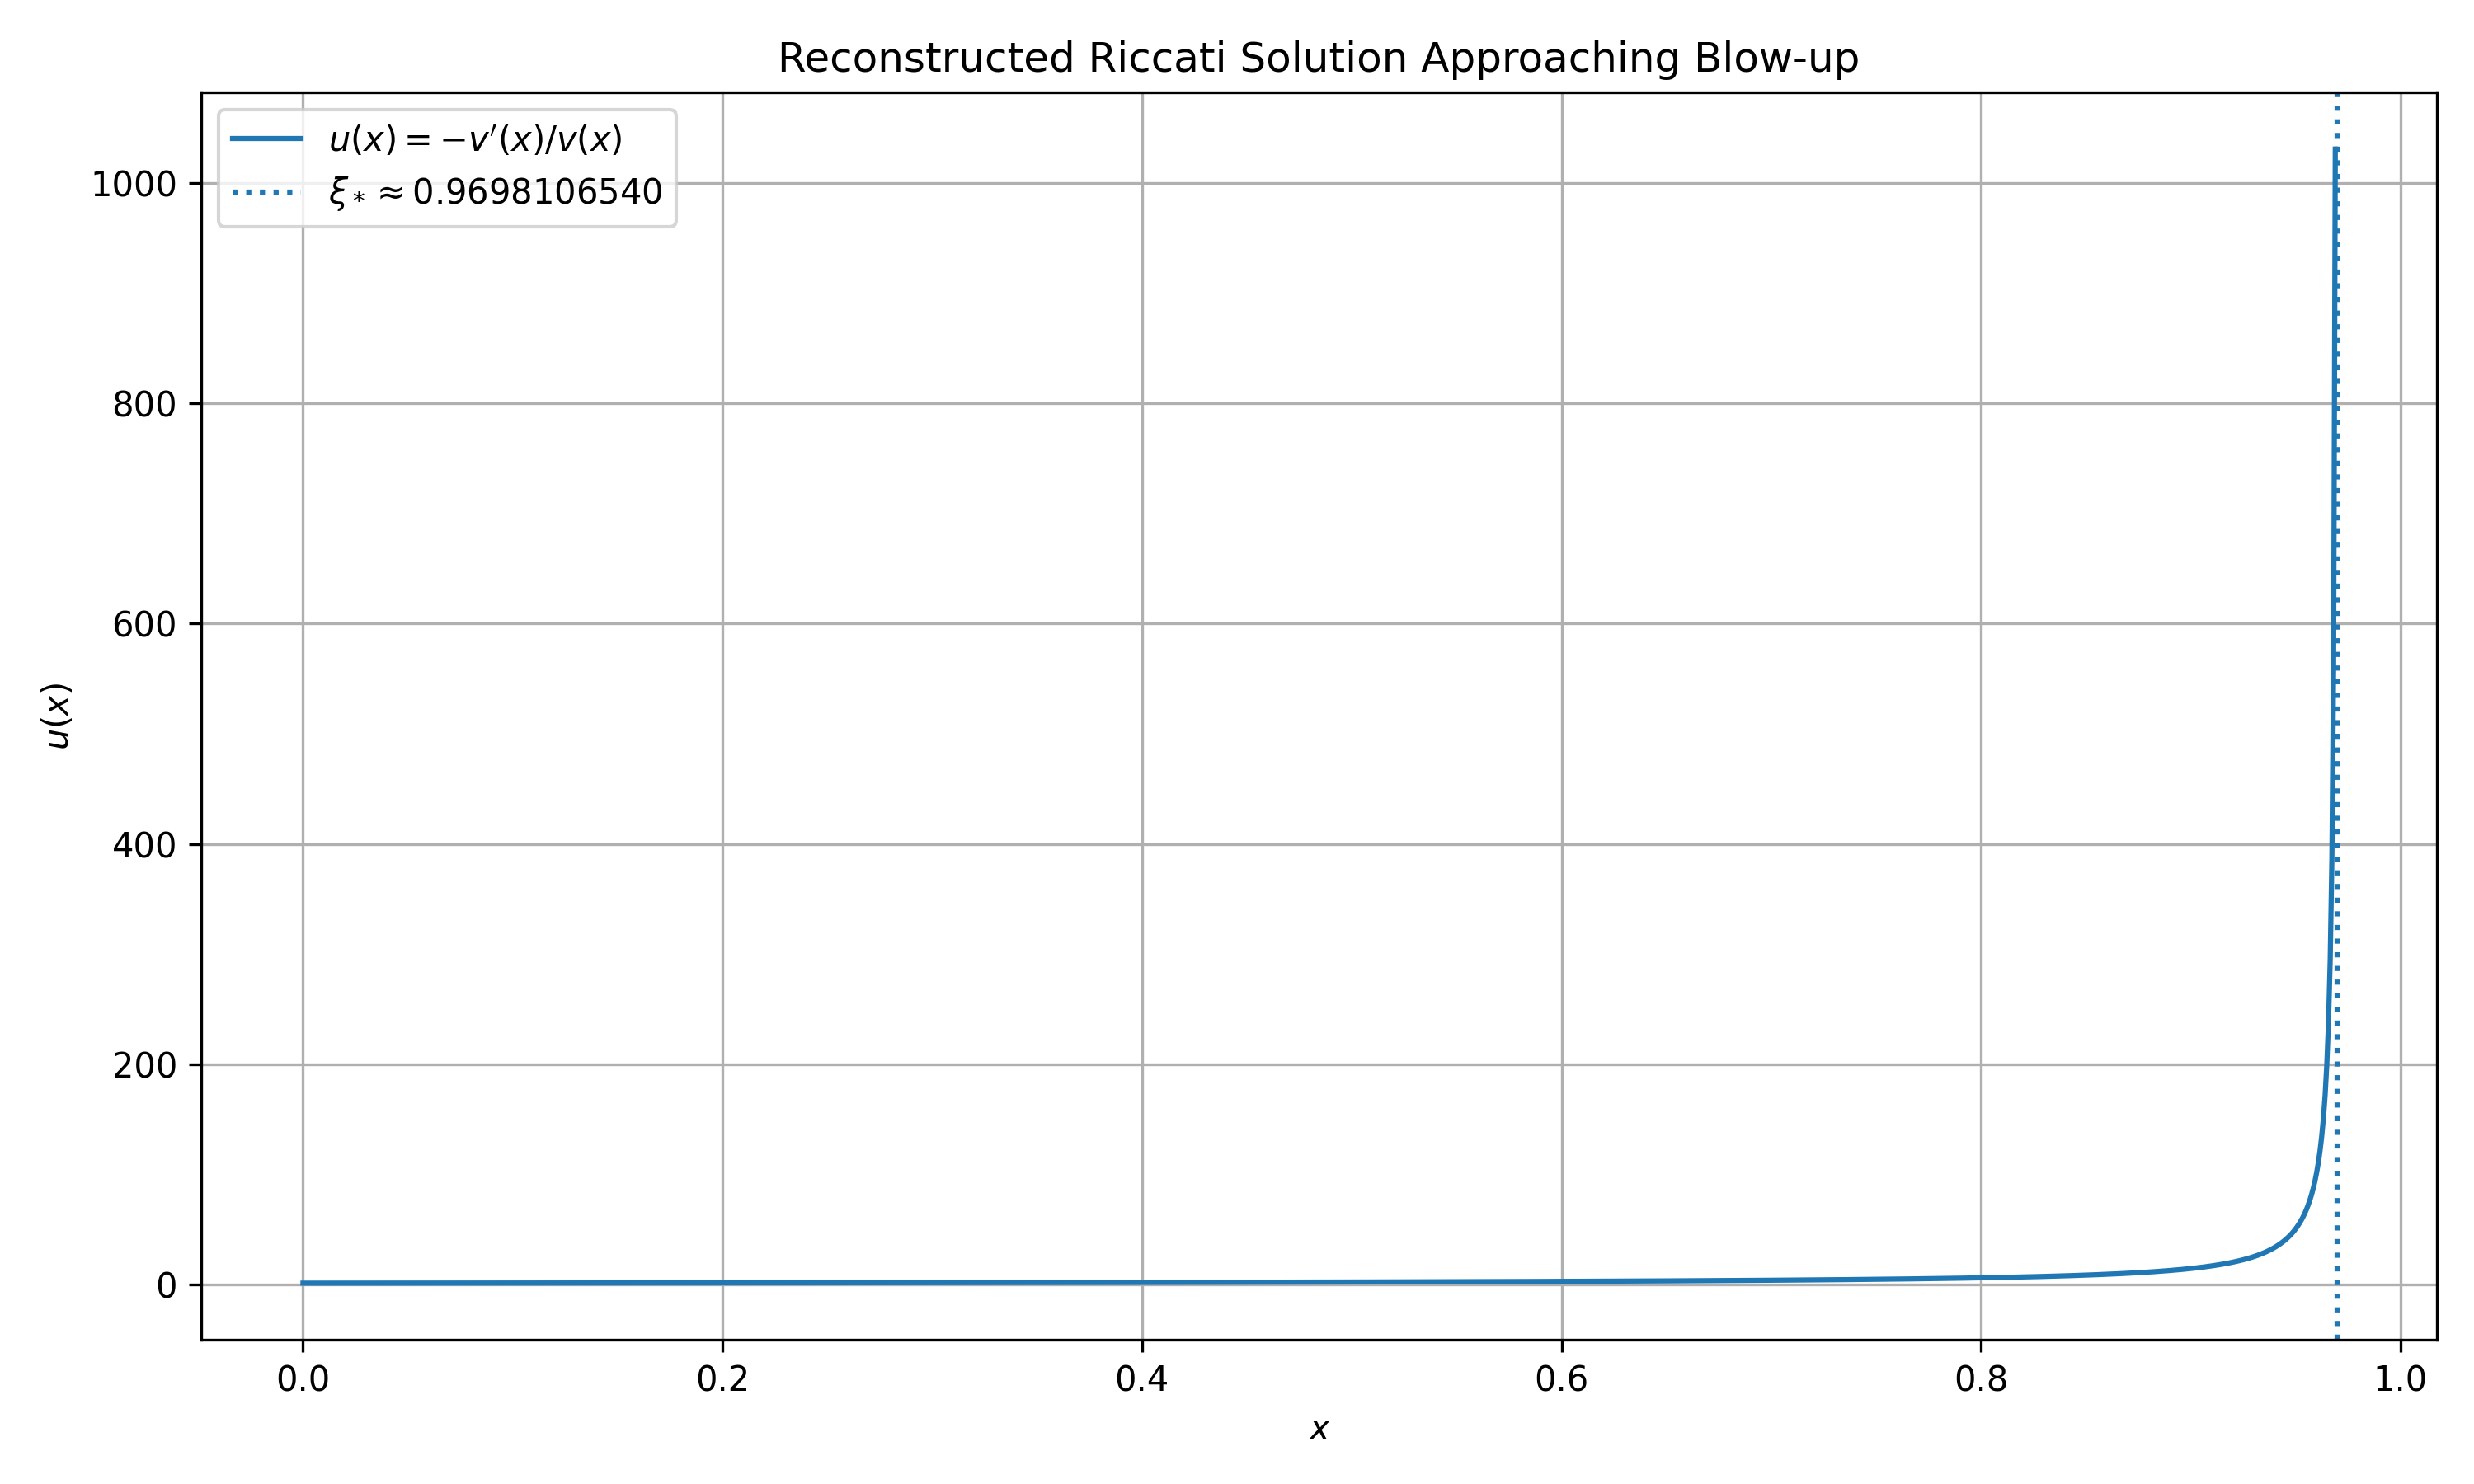
\includegraphics[height=0.53\textheight,keepaspectratio]{beamer_assets/riccati_reconstructed_blowup.png}
\end{frame}

\begin{frame}{From the Computed Stopping Time to Koopman Eigenfunctions}
\footnotesize
For the lifted Riccati system,
\[
F(x,y)=(1,x^2+y^2),
\qquad
\boxed{Kg=g_x+(x^2+y^2)g_y.}
\]
In this Riccati example, the relevant first zero \(\xi_*(s,y)\) is simple and varies continuously with the initial data; hence \(m(s,y)=\xi_*(s,y)-s\) is continuous.

For any real \(\lambda>0\), define
\[
\boxed{\phi_\lambda(s,y)=e^{-\lambda m(s,y)}.}
\]
Using the remaining-lifetime identity,
\[
\phi_\lambda(\flow(t,z))=e^{\lambda t}\phi_\lambda(z),
\qquad 0\le t<m(z),\qquad z=(s,y).
\]
Formally, on the generator domain,
\[
\boxed{K\phi_\lambda=\lambda\phi_\lambda.}
\]

\begin{alertblock}{Computational payoff}
Event detection computes \(m(s,y)\), so the same computation gives numerical values of the Koopman eigenfunction \(\phi_\lambda\).
\end{alertblock}
\end{frame}


% ------------------------------------------------------------
% 27. Synthesis
% ------------------------------------------------------------
\begin{frame}{How the Pieces Fit Together}
\begin{center}
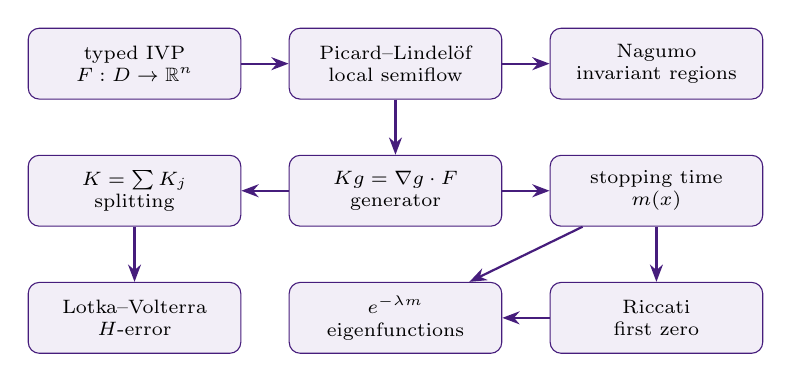
\begin{tikzpicture}[node distance=7mm and 6mm, every node/.style={align=center,font=\scriptsize}]
\node[draw=LSUPurple,fill=SoftPurple,rounded corners,minimum width=2.7cm,minimum height=0.9cm] (ivp) {typed IVP\\\(F:D\to\R^n\)};
\node[draw=LSUPurple,fill=SoftPurple,rounded corners,right=of ivp,minimum width=2.7cm,minimum height=0.9cm] (well) {Picard--Lindel\"of\\local semiflow};
\node[draw=LSUPurple,fill=SoftPurple,rounded corners,right=of well,minimum width=2.7cm,minimum height=0.9cm] (nag) {Nagumo\\invariant regions};
\node[draw=LSUPurple,fill=SoftPurple,rounded corners,below=of well,minimum width=2.7cm,minimum height=0.9cm] (gen) {\(Kg=\nabla g\cdot F\)\\generator};
\node[draw=LSUPurple,fill=SoftPurple,rounded corners,left=of gen,minimum width=2.7cm,minimum height=0.9cm] (split) {\(K=\sum K_j\)\\splitting};
\node[draw=LSUPurple,fill=SoftPurple,rounded corners,right=of gen,minimum width=2.7cm,minimum height=0.9cm] (stop) {stopping time\\\(m(x)\)};
\node[draw=LSUPurple,fill=SoftPurple,rounded corners,below=of split,minimum width=2.7cm,minimum height=0.9cm] (lv) {Lotka--Volterra\\\(H\)-error};
\node[draw=LSUPurple,fill=SoftPurple,rounded corners,below=of stop,minimum width=2.7cm,minimum height=0.9cm] (ric) {Riccati\\first zero};
\node[draw=LSUPurple,fill=SoftPurple,rounded corners,below=of gen,minimum width=2.7cm,minimum height=0.9cm] (eig) {\(e^{-\lambda m}\)\\eigenfunctions};

\draw[-{Stealth[length=2.2mm]},thick,LSUPurple] (ivp)--(well);
\draw[-{Stealth[length=2.2mm]},thick,LSUPurple] (well)--(nag);
\draw[-{Stealth[length=2.2mm]},thick,LSUPurple] (well)--(gen);
\draw[-{Stealth[length=2.2mm]},thick,LSUPurple] (gen)--(split);
\draw[-{Stealth[length=2.2mm]},thick,LSUPurple] (gen)--(stop);
\draw[-{Stealth[length=2.2mm]},thick,LSUPurple] (split)--(lv);
\draw[-{Stealth[length=2.2mm]},thick,LSUPurple] (stop)--(ric);
\draw[-{Stealth[length=2.2mm]},thick,LSUPurple] (stop)--(eig);
\draw[-{Stealth[length=2.2mm]},thick,LSUPurple] (ric)--(eig);
\end{tikzpicture}
\end{center}

\begin{alertblock}{One mathematical story}
Well-posedness creates the local evolution, invariance controls where it can move, the generator produces the splitting, and stopping times connect finite-time blow-up to computable observable/eigenfunction information.
\end{alertblock}
\end{frame}

% ------------------------------------------------------------
% 28. Reproducibility
% ------------------------------------------------------------
\begin{frame}{Computational Reproducibility}
The complete Python programs and supporting files used for the numerical experiments are maintained in a public repository:

\vspace{0.55em}
\begin{center}
\large
\href{https://github.com/matthewxclarkjr/ThesisODE2026}{\textcolor{LSUPurple}{\texttt{github.com/matthewxclarkjr/ThesisODE2026}}}
\end{center}

\vspace{0.45em}
The repository includes:
\begin{itemize}
  \item \texttt{lotka\_volterra\_lab.py},
  \item \texttt{LVinput.txt} for reproducible Lotka--Volterra runs,
  \item the Riccati zero-detection / stopping-time script,
  \item supporting visualization scripts,
  \item \texttt{README.md} and \texttt{requirements.txt}.
\end{itemize}

\begin{alertblock}{Thesis / repository split}
The thesis explains the mathematics and numerical conclusions; the repository provides the complete executable computational materials.
\end{alertblock}
\end{frame}

% ------------------------------------------------------------
% 29. Conclusions
% ------------------------------------------------------------
\begin{frame}{Conclusions}
\small
\begin{itemize}
  \item Picard--Lindel\"of supplies a unique local semiflow on the natural domain \(0\le t<m(x)\).
  \item Nagumo's theorem gives a practical boundary test for positively invariant closed regions.
  \item For differentiable observables, \(Kg=\nabla g\cdot F\); its coordinate decomposition \(K=\sum K_j\) produces the natural splitting used in the numerical schemes.
  \item In the Lotka--Volterra laboratory, preservation of \(H\) provides a structural error diagnostic. The comparison uses low-order splitting schemes and an adaptive reference solver.
  \item Stopping times are extended-real-valued and lower semicontinuous; they may fail to be continuous because of domain exit.
  \item For the Riccati example, nonlinear blow-up is converted into a linear first-zero problem:
  \[
  \boxed{m(s,y)=\xi_*(s,y)-s.}
  \]
  The computed stopping time also gives computable Koopman eigenfunction values \(e^{-\lambda m(s,y)}\).
\end{itemize}
\end{frame}

% ------------------------------------------------------------
% 30. References
% ------------------------------------------------------------
\begin{frame}{Selected References}
\footnotesize
\setlength{\parindent}{0pt}
\setlength{\parskip}{0.42em}

\hangindent=1.5em\hangafter=1
Coddington, E. A., and N. Levinson. \emph{Theory of Ordinary Differential Equations}. McGraw--Hill, 1955.

\hangindent=1.5em\hangafter=1
Teschl, G. \emph{Ordinary Differential Equations and Dynamical Systems}. AMS, 2012.

\hangindent=1.5em\hangafter=1
Engel, K.-J., and R. Nagel. \emph{One-Parameter Semigroups for Linear Evolution Equations}. Springer, 2000.

\hangindent=1.5em\hangafter=1
Banjara, A. \emph{Higher Order Operator Splitting Schemes with Complex Coefficients and Applications}. Doctoral dissertation, LSU, 2024.

\hangindent=1.5em\hangafter=1
Neubrander, F. \emph{Ordinary Differential Equations, Semiflows, and Semigroups}. Unpublished lecture notes for MATH 7320, LSU, Spring 2026.
\end{frame}

% ------------------------------------------------------------
% 31. Questions
% ------------------------------------------------------------
{\setbeamercolor{background canvas}{bg=LSUPurple}
\begin{frame}[plain]
\vfill
\centering
{\color{white}\Huge\bfseries Questions?\par}
\vspace{1em}
{\color{LSUGold}\Large Thank you.\par}
\vfill
\end{frame}}

\appendix

\begin{frame}{Backup: Riccati Linearization Details}
\footnotesize
Fix \((s,y)\in\R^2\). For \(x\ge s\),
\[
u'(x)=x^2+u(x)^2,\qquad u(s)=y.
\]
Set
\[
\boxed{u(x)=-\frac{v'(x)}{v(x)}}.
\]
Differentiate:
\[
u'
=
-\frac{v''}{v}
+
\left(\frac{v'}{v}\right)^2.
\]
Since \(u^2=(v'/v)^2\), substitution into the Riccati equation gives
\[
-\frac{v''}{v}=x^2,
\]
so
\[
\boxed{v''(x)+x^2v(x)=0.}
\]
Normalize \(v(s)=1\). From \(u(s)=y\),
\[
\boxed{v'(s)=-y.}
\]
Thus the detailed calculation gives exactly the linear IVP stated on slide 27.
\end{frame}

\begin{frame}{Backup: Why the First Zero Gives Riccati Blow-up}
\footnotesize
Let \(\xi_*>s\) be the first zero of the nontrivial solution \(v\). Since \(v(s)=1\), \(v\not\equiv0\).

If
\[
v(\xi_*)=v'(\xi_*)=0,
\]
uniqueness for the linear IVP would force \(v\equiv0\), a contradiction. Therefore
\[
\boxed{v'(\xi_*)\neq0,}
\]
so the zero is simple.

Near \(\xi_*\),
\[
v(x)=v'(\xi_*)(x-\xi_*)+o(|x-\xi_*|),
\]
and hence
\[
-\frac{v'(x)}{v(x)}
\sim
-\frac{1}{x-\xi_*}.
\]
Thus
\[
u(x)=-\frac{v'(x)}{v(x)}\longrightarrow+\infty
\qquad (x\uparrow\xi_*).
\]
Because \(x=s+\tau\),
\[
\boxed{m(s,y)=\xi_*-s.}
\]
\end{frame}

\begin{frame}{Backup: Why a First Zero Exists}
\footnotesize
For
\[
v''(x)+x^2v(x)=0,
\]
fix \(R>0\). On \(x\ge R\),
\[
x^2\ge R^2.
\]
Sturm comparison with
\[
z''+R^2z=0
\]
shows that a nontrivial solution of \(v''+x^2v=0\) cannot remain zero-free forever to the right; a zero occurs in finite distance.

\begin{alertblock}{Role of Sturm comparison}
This establishes the existence of the first zero \(\xi_*(s,y)>s\). The preceding backup slide gives the simple-zero and pole argument showing that this zero is the Riccati blow-up location.
\end{alertblock}
\end{frame}

\begin{frame}{Backup: Formal Tangent-Cone Definition}
\small
For a closed set \(\Omega\subset\R^n\) and \(x\in\Omega\),
\[
\boxed{
T_\Omega(x)
=
\left\{
v\in\R^n:
\liminf_{h\downarrow0}
\frac{\operatorname{dist}(x+h v,\Omega)}{h}=0
\right\}.
}
\]
This cone contains directions that are tangent to \(\Omega\) or point inward to first order.

For regular inequality constraints
\[
\Omega=\{x:g_j(x)\le0\},
\]
the tangent condition is equivalent on active boundaries to
\[
\nabla g_j(x)\cdot F(x)\le0,
\]
which is the boundary test used in the main presentation.
\end{frame}

\begin{frame}{Backup: Local Koopman Domain and Function-Space Caveat}
\small
For a local semiflow,
\[
\mathcal D=\{(t,x):0\le t<m(x)\}.
\]
Thus \(g(\sigma(t,x))\) is only defined when \((t,x)\in\mathcal D\).

The main presentation therefore uses the pointwise statement:
\[
\boxed{
\text{for fixed }x\text{ and }0\le t<m(x),\quad
g\mapsto g(\sigma(t,x))
\text{ is linear}.
}
\]

No particular Banach function space is fixed in the main argument. If one chooses a specific local-semigroup framework, additional operator-theoretic structure can be developed, but that is not required for the calculations presented here.
\end{frame}

\begin{frame}{Backup: Step-Size Refinement Table}
\centering
\scriptsize
\setlength{\tabcolsep}{3.0pt}
\renewcommand{\arraystretch}{1.25}
\begin{tabular}{ccccc}
\toprule
\(h\) & Forward Euler & Lie--Trotter & Strang & \texttt{solve\_ivp} \\
\midrule
0.01  & 161.6626980950\% & -1.2478784951\% & -0.0023496487\% & -0.0000001293\% \\
0.005 & 67.7244617696\%  &  0.1034928563\% & -0.0006536800\% & -0.0000001293\% \\
0.001 & 10.3619531982\%  & -0.0865717147\% & -0.0000269765\% & -0.0000001293\% \\
\bottomrule
\end{tabular}

\vspace{0.7em}
\begin{alertblock}{How to read the last column}
The listed \(h\) is the fixed step used by forward Euler, Lie--Trotter, and Strang. \texttt{solve\_ivp} is adaptive: the output grid changes, but its internal steps are controlled by tolerances. The nearly unchanged reference error is therefore not a fixed-step convergence experiment for \texttt{solve\_ivp}.
\end{alertblock}
\end{frame}

\begin{frame}{Backup: Spectral Extension}
\small
The main talk uses real \(\lambda>0\). In the standard Koopman--Lie framework for the globally defined Riccati vector field, the same construction extends to complex \(\lambda\) with
\[
\operatorname{Re}\lambda>0.
\]
Define
\[
\phi_\lambda(z)=e^{-\lambda m(z)}.
\]
Then along admissible trajectories,
\[
\phi_\lambda(\sigma(t,z))
=
e^{\lambda t}\phi_\lambda(z),
\]
and formally
\[
K\phi_\lambda=\lambda\phi_\lambda.
\]

This is the spectral connection highlighted in Neubrander's lecture notes: finite stopping time produces Koopman eigenfunctions in the right half-plane.
\end{frame}

\begin{frame}{Backup: Example 3 Visual (for Consideration)}
\footnotesize
\begin{columns}[T,onlytextwidth]
\column{0.38\textwidth}
\[
\Gamma=\{(x,0):x\ge1\},
\qquad
\Omega=\R^2\setminus\Gamma,
\qquad
F(x,y)=(1,0).
\]
\[
\mstop(x_0,y_0)=
\begin{cases}
+\infty, & y_0\neq0,\\
1-x_0, & y_0=0,\ x_0<1.
\end{cases}
\]
For
\[
z_n=\left(x_0,\frac1n\right)\to(x_0,0),
\]
we get
\[
\mstop(z_n)=+\infty,
\qquad
\mstop(x_0,0)=1-x_0<\infty.
\]
Hence \(m\) is not continuous, but the jump is upward, so lower semicontinuity is preserved.

\column{0.60\textwidth}
\centering
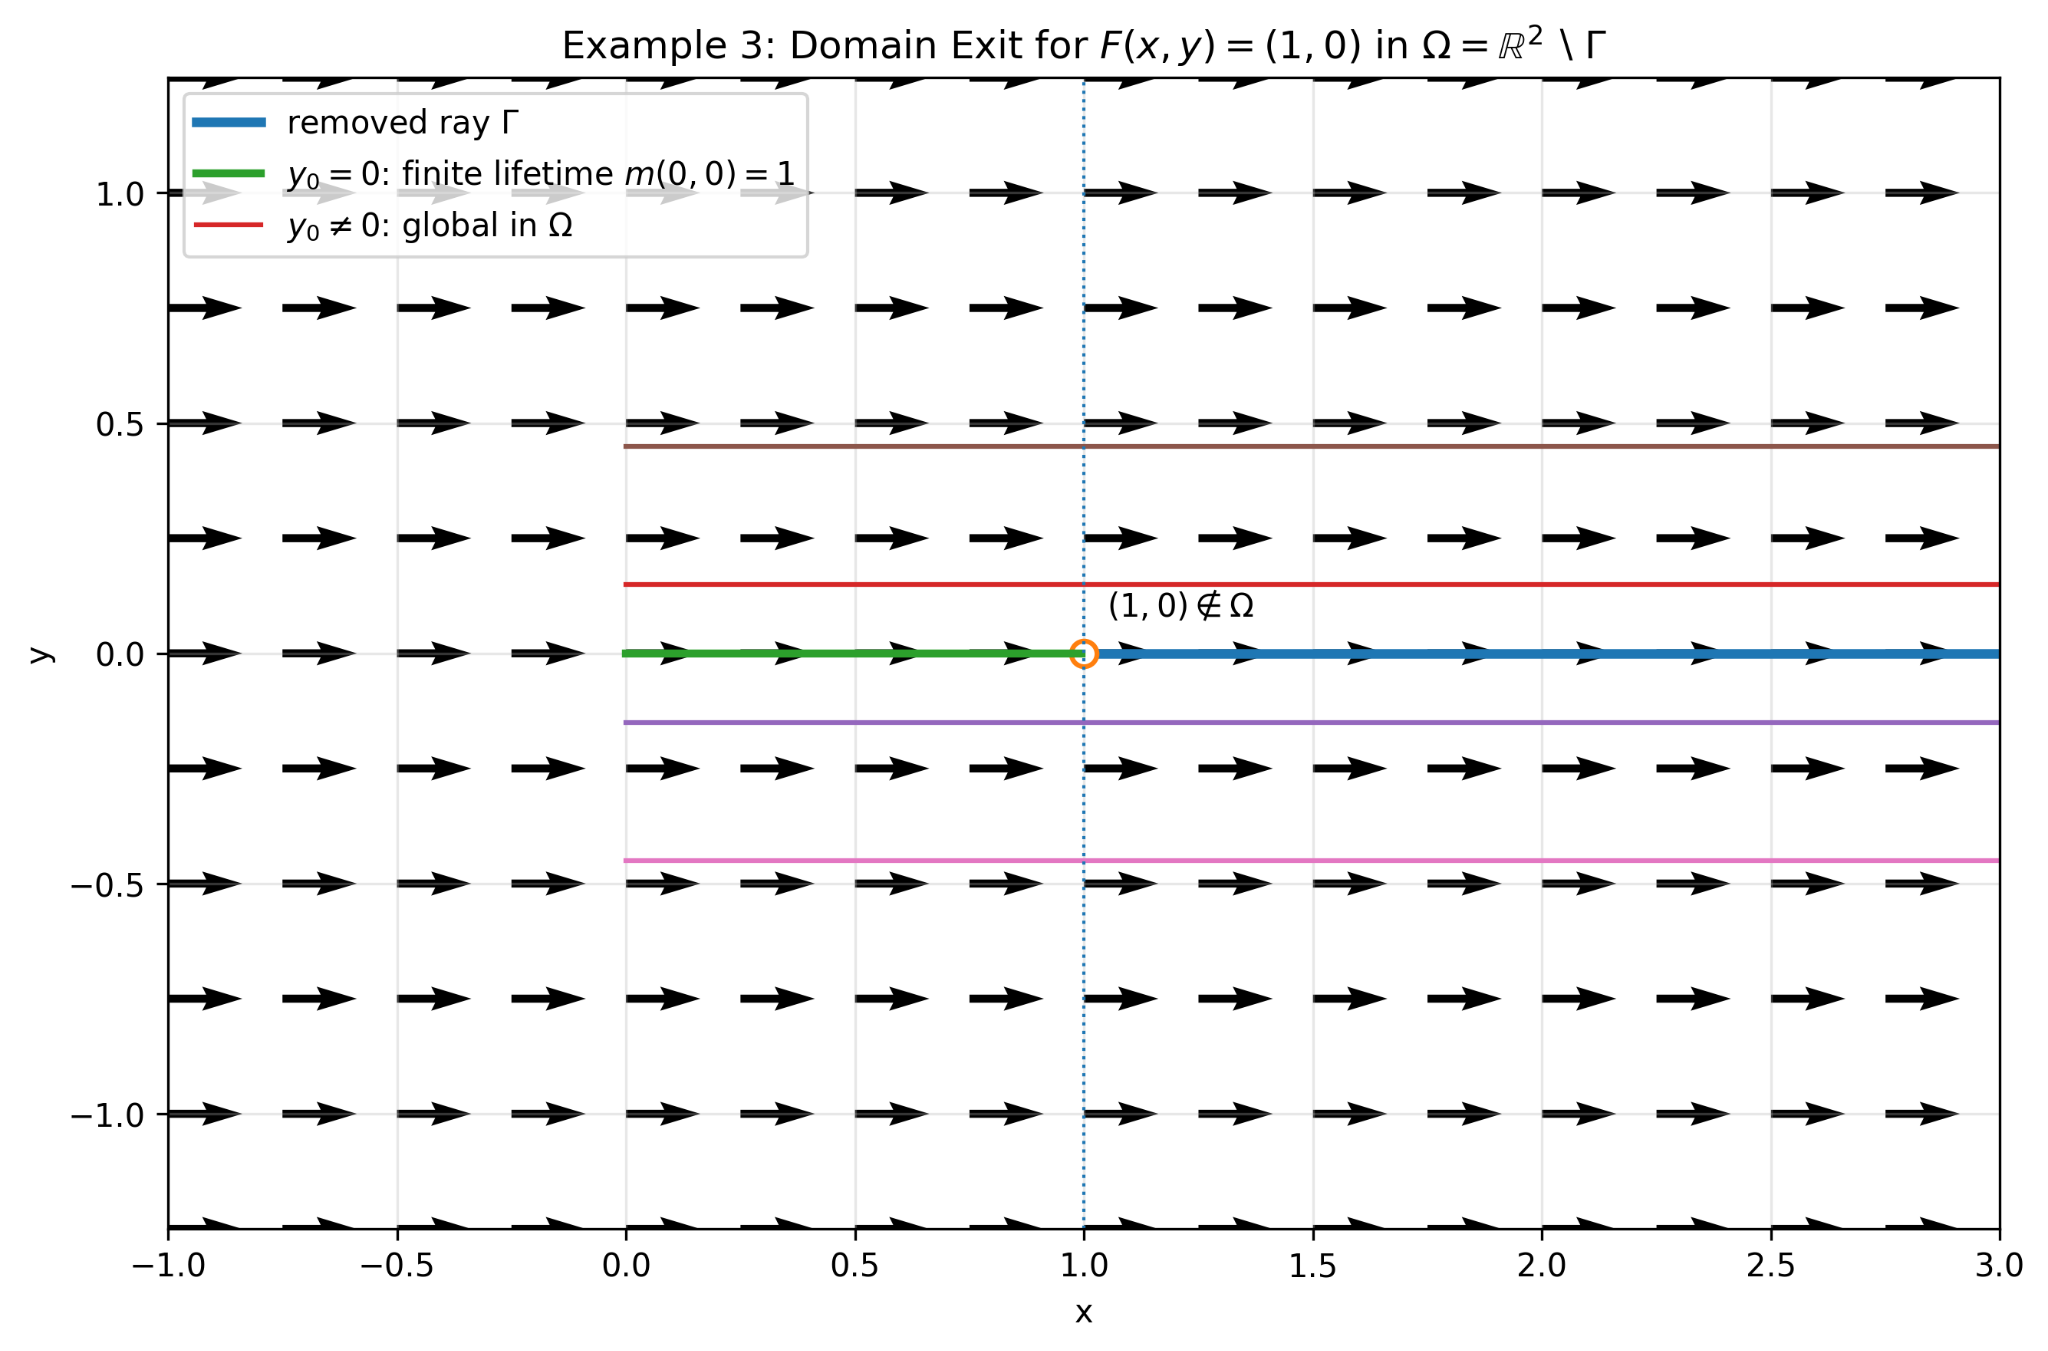
\includegraphics[width=\linewidth]{beamer_assets/discontinuous_stopping_time_vector_field.png}
\end{columns}
\end{frame}



\end{document}
